% REMEMBER: You must not plagiarise anything in your report. Be extremely careful.

\documentclass{l4proj}


%
% put any additional packages here
%
\usepackage{pgf-umlsd}
\usepackage{scalefnt}
\usepackage{tikz}
\usepackage{float}
\usepackage{pdfpages}
\usepackage{multirow}

\setcitestyle{square}
\begin{document}


%==============================================================================
%% METADATA
\title{Where is ECN stripped on the network?}
\author{Myles Lamb}
\date{April 12, 2021}

\maketitle

%==============================================================================
%% ABSTRACT
\begin{abstract}
    
 Explicit Congestion Notification (ECN) allows devices on the network to signal incipient congestion before a congestive loss occurs. However, devices on the network have presented deployment issues for features such as ECN through applying modifications to packets that are destructive to ECN signalling. This paper investigates where network devices alter ECN Capable Transport (ECT) code points. To achieve this, we implement a new network analysis tool. We subsequently conduct a medium-scale deployment of the tool to gather various measurements from the network to ascertain the current state of affairs of the treatment of ECN on the network. Key findings include that there does not appear to be any particular inhibitors to the deployment of ECN within Quic. Additionally, we find that the transport protocol in use generally does not influence the behaviour of devices on the network.
    
\end{abstract}

\chapter*{Acknowledgements}

I would like to thank my advisor, Dr Colin Perkins, for his exceptional guidance across this project's duration despite the adverse circumstances that this body of work was produced within.

%==============================================================================

\def\consentname {Myles Lamb} % your full name
\def\consentdate {April 12 2021} % the date you agree

\educationalconsent


%==============================================================================
\tableofcontents

%==============================================================================
%% Notes on formatting
%==============================================================================
% The first page, abstract and table of contents are numbered using Roman numerals and are not
% included in the page count. 
%
% From now on pages are numbered
% using Arabic numerals. Therefore, immediately after the first call to \chapter we need the call
% \pagenumbering{arabic} and this should be called once only in the document. 
%
% The first Chapter should then be on page 1. You are allowed 40 pages for a 40 credit project and 20 pages for a 
% 20 credit report. This includes everything numbered in Arabic numerals (excluding front matter) up
% to but excluding the appendices and bibliography.
%
% You must not alter text size (it is currently 10pt) or alter margins or spacing.
%
%
%==================================================================================================================================
%
% IMPORTANT
% The chapter headings here are **suggestions**. You don't have to follow this model if
% it doesn't fit your project. Every project should have an introduction and conclusion,
% however. 
%
%==================================================================================================================================


\chapter{Introduction}
\label{chap:introduction}

% reset page numbering. Don't remove this!
\pagenumbering{arabic} 

This chapter will motivate developing a new network analysis tool to investigate the adoption of Explicit Congestion Notification (ECN). Additionally, we investigate the frequency and location of devices that alter ECN expressions on the network path. The following chapters will discuss various aspects of the project, such as the design and implementation of the network analysis tool and analysis of the results of a medium-scale deployment of the previously developed tool.

Initially defined in RFC 3168, ECN is an extension to the Internet Protocol (IP) and some higher-level protocols such as Transmission Control Protocol (TCP). ECN allows devices on the network to signal incipient congestion to end-hosts allowing them to respond accordingly through reducing sending rates before packet loss due to network congestion occurs\cite{rfc3168}.

The deployment of ECN has been hampered due to devices negatively interacting with packets that attempt to utilise ECN. Such as resetting connections that try to negotiate ECN or remarking packets that indicate ECN capable transport\cite{floyd_inappropriate_2002}, ultimately leading to a lack of faith in the technology. Whilst these issues have lessened in prevalence over time \cite{trammell_enabling_2015}, there has been a renewed interest in the deployment of ECN through its integration with Quic, a new transport protocol operating over UDP\cite{johansson_ecn_2017}. We additionally recognise the growing need to reduce queuing delays across modern networks, given the increasing prevalence of real-time traffic. This presents ECN markings' preservation across the network as critical for managing the network's continued development. To the best of our knowledge, this paper presents the first set of findings relating to the deployment of ECN within Quic, additionally illustrating a new technical method for measuring on path removal of ECT code points to TCP-based hosts.

We present the aims of this paper as follows; We intend to investigate the overall adoption of ECN. Additionally, we explore where as well as how often devices on the network modify the expressions of ECT code points on traffic on the network. We also seek to discern whether the internet protocol version or choice of transport layer substrate influences the remarking behaviour of devices on the network. We additionally incorporate new protocols that support ECN, such as Quic. Lastly, we investigate whether the available ECT code points experience different remarking behaviours from devices on the network. To achieve this, we will; Devise a suitable experimental methodology to gather appropriate measurements from the network (Section \ref{chap:design}). We then design and implement a network analysis tool supporting the goals of the experimental methodology (Section \ref{chap:design} and Section \ref{chap:implementation}). Lastly, we evaluate the data produced by the network analysis tool through a medium-scale deployment across numerous geographically distributed hosts (Section \ref{chap:evaluation}).

\clearpage


%==================================================================================================================================
\chapter{Background}
\label{chap:background}

This chapter discusses the fundamentals of ECN as a technology and presents the contributions of previous works. Identifying areas for elaboration in existing research.
\addtocontents{toc}{\protect\setcounter{tocdepth}{1}}

\section{Overview of ECN}

% Explain why routers drop packets, and why hosts use congestive loss as a signal for congestion %

% Explain why remarking on AS boundaries %

Routers on the network function through a buffering and forwarding approach, Packets arrive on a network interface and are buffered by a given device. Devices typically use a queue like data structure in memory. Given the characteristics of the packets that arrive on a given interface, decisions are made on where to forward the given traffic to. However, if packets are arriving faster at a given router than are being forwarded, the queue of packets should grow. We have that for a given device on the network, that memory is finite. Hence, once the buffer available for packets is exhausted, the device should begin to discard packets. Typically, end-hosts on the network recognise that packets they have sent have been dropped on the network and typically reduce their sending rates to allow the responsible device to recover. Packet losses in this context are referred to as loss-based congestion signals.

The traditional end-to-end approach to congestion control employed within transport protocols such as TCP results in end hosts inferring congestion on the network through loss based congestion signals. Whilst protocols such as TCP have managed well through the use of congestion signals, such as packet loss. With the advent of mobile computing and the internet of things, with implied wireless communication. It is not clear that loss based congestive signals are the most suitable.
ECN is a mechanism that allows for devices on the network to signal incipient congestion to end hosts before a congestive loss occurs\citep{rfc3168}. This enables routers utilising Active Queue Management (i.e. Random Early Detection) to mark packets when congestion is experienced. Recipients observing these markings inform the sender of their observation, allowing them to reduce their sending rate before a congestive loss occurs. Avoiding congestive loss through ECN mitigates negative aspects of packet loss on the network; this includes head-of-line blocking for protocols that provide an in-order delivery service model in the case of TCP. Alternatively, providing benefits to service quality for protocols that do not re-transmit lost packets, such as Real-time Transport Protocol (RTP) \citep{rfc6679}.
ECN is implemented through two bits of the IPv4/IPv6 header. Namely, the two least significant bits of the Traffic Class byte, with the other 6 bits constituting the differentiated services code point (DSCP). These two bits of the IP header are used to signify whether a given transport is ECN capable and whether congestion has been experienced on the network. We have four potential bit patterns using these bits, called ECT (ECN capable transport) code points. These bit patterns are interpreted as follows, 00 = not ECN capable, 10 = ECT(0), 01 = ECT(1), 11 = CE (congestion experienced).

We may note that both ECT(0) and ECT(1) can be used to signal a given transport is ECN capable, and both are to be treated equivalently by devices on the network \citep{rfc3168}. Furthermore, if a device on the network does not leverage the ECN field, it should not modify it. However, the first standard presenting ECN was introduced in 2001. Before its' introduction, the bits that constitute the ECN field occupy part of the legacy ToS (Type of Service) byte. With the presence of older equipment on the network continuing to use ToS semantics, we gain some insight into why devices on the network interact poorly with ECN(\cite{kuhlewind_state_2013}).

Lastly, the CE code point is used by devices on the network to signal that congestion is incipient on a given device. Routers that implement ECN related functionality typically employ an algorithm such as Random early detection (RED) to produce a probability of dropping packets in the future. Suppose this probability is over a given threshold. In that case, the router will mark packets that indicate ECN capable transport with the congestion experienced code point as a means to inform senders to reduce their sending rates. To avoid the congested router's associated buffer from overflowing resulting in a congestive loss.

\subsection{Historic use of ToS and its implications}

As previously mentioned, the IP header's bits that constitute the ECN field did not always serve this purpose. Historically, these bits formed part of the ToS byte, which served many related purposes over the years of its use—initially presented by \citep{rfc791} and further updated numerous times in the following years. It was primarily used to identify traffic precedence and provide mechanisms to request specific treatment on the network, such as low latency or high reliability. This field was typically employed on Autonomous Systems (ASs) borders. ASs are typically large networks that conform to a singular routing policy. Packets entering an AS would typically be marked with a given ToS value describing the required treatment of traffic entering the AS. They may additionally remark the ToS field as traffic leaves a given AS, known as boundary remarking. Whilst efforts were made to ensure some level of compatibility between ToS and the later introduced DSCP in RFC 3168, such as maintaining the IP Precedence aspect of ToS\citep{rfc3168}. This could not be extended to ECN, a concept conceived after the deprecation of the ToS field. The bits that constitute ECN were either unused and set to zero as defined in RFC 791\citep{rfc791}. Alternatively, in RFC 1349, the rightmost bit was always zeroed, referenced as a "Must-be-zero" bit\citep{rfc1349}. Hence, as the bits that constitute the modern ECN field have been redefined several times over previous years, we can potentially have many different interpretations for the ECN field. Given the existence of older networking equipment that continues to use the ToS field as defined in \cite{rfc791} or later definitions. For instance, \cite{custura_exploring_2017} demonstrated several devices on the network that continue to use ToS based semantics. With many exhibiting destructive behaviours towards ECN.

\section{ECN Within TCP}
\label{sec:ecntcp}

Support for ECN under TCP was defined in RFC 3168\cite{rfc3168}. When ECN is utilised with TCP, hosts must first negotiate its use at the beginning of the TCP connection during the SYN-ACK exchange as part of TCP connection establishment. ECN under TCP utilises two previously reserved bits of the TCP header. Namely the ECE (ECN Echo) and the CWR (Congestion window reduced) bits. Hosts may negotiate ECN by setting the ECE (ECN-echo) and CWR bits of the TCP header on the initiating SYN of the TCP handshake. If the receiving host also desires to use ECN, a SYN-ACK with the ECE bit set will be returned. Subsequent data segments sent during the connection should be marked with either ECT(0) or ECT(1) on the IP header to indicate ECN capable transport. When congestion is experienced on a node on the network, the network device should mark a given packet with the ECE code point. End hosts receiving a packet with the CE code point set should respond by setting the ECE bit in the TCP header on the following segment sent during the connection. The sending host then indicates the receipt of a segment with ECE bit set, by setting the CWR bit in the TCP header of the following segment sent, as well as responding with respect to the congestion control algorithm in use as if packet loss had occurred, this process is summarised in figure \ref{fig:ecn_tcp}.



\begin{center}
    \begin{figure}[H]
            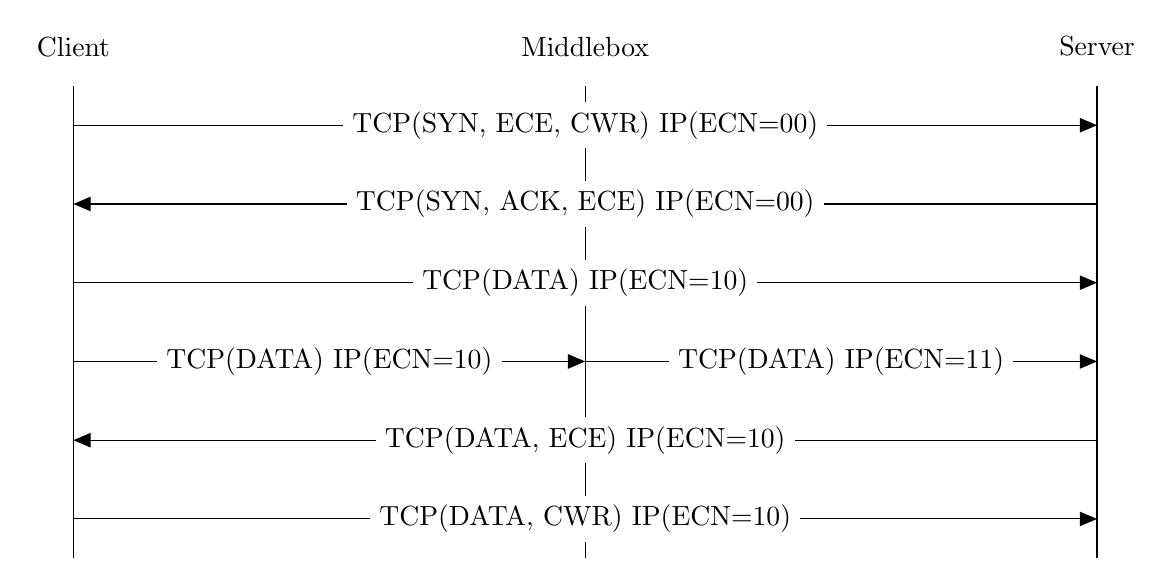
\begin{tikzpicture}
            
            \draw (0,0) -- (0, 6);
            \draw (6.5,0) -- (6.5, 6);
            \draw (13,0) -- (13, 6);
            \node at (0,6.5) {Client};
            \node at (6.5,6.5) {Middlebox};
            \node at (13,6.5) {Server};
            
            \draw [arrows={-triangle 45}]
            (0, 5.5) -- (13, 5.5) node [midway, fill=white, text centered]
            { TCP(SYN, ECE, CWR)  IP(ECN=00)};
            
            \draw [arrows={triangle 45-}]
            (0, 4.5) -- (13, 4.5) node [midway, fill=white, text centered]
            { TCP(SYN, ACK, ECE)  IP(ECN=00)};
            
            \draw [arrows={-triangle 45}]
            (0, 3.5) -- (13, 3.5) node [midway, fill=white, text centered]
            { TCP(DATA)  IP(ECN=10)};
            
            \draw [arrows={-triangle 45}]
            (0, 2.5) -- (6.5, 2.5) node [midway, fill=white, text centered]
            { TCP(DATA)  IP(ECN=10)};
            
            \draw [arrows={-triangle 45}]
            (6.5, 2.5) -- (13, 2.5) node [midway, fill=white, text centered]
            { TCP(DATA)  IP(ECN=11)};
            
            \draw [arrows={triangle 45-}]
            (0, 1.5) -- (13, 1.5) node [midway, fill=white, text centered]
            { TCP(DATA, ECE)  IP(ECN=10)};
            
            \draw [arrows={-triangle 45}]
            (0, 0.5) -- (13, 0.5) node [midway, fill=white, text centered]
            { TCP(DATA, CWR)  IP(ECN=10)};
            
            \end{tikzpicture}
        \caption{Diagrammatic representation of the operation of ECN with TCP/IP with a congested link on the network. When a given device on the network experiences congestion, it remarks the ECN field of packets indicating ECN capable transport to the CE code point. Sending hosts respond by reducing their sending rates as if a loss on the network had occurred. TCP acks have been omitted for the sake of brevity.}
    \label{fig:ecn_tcp}
    \end{figure}
\end{center}
\section{ECN Within UDP}

ECN is not directly used with UDP. The actual operation of ECN with UDP is deferred to the context of a higher layer protocol, such as RTP, or Quic, which utilise UDP as their transport substrate. In the following text, we discuss the operation of ECN within Quic, one of the protocols investigated in this paper. Quic introduced the notion of ECN support with an IETF draft discussing its intended operation\citep{johansson_ecn_2017}. Whilst Quic is still in development as a protocol (lacking an RFC), we summarise the function of ECN under Quic within IETF draft 29\cite{thomson_quic_2020} (the variant of Quic used in this paper).

% Elaborate %

When ECN is utilised with Quic, the sender must first determine whether both the path and the end host support ECN marking. Support for ECN marking is defined as whether ECT code points are not cleared on the network path and that packets setting ECT code points are not dropped. Additionally, we require that the end host can view and set the ECN field on the IP header. This is verified by sending early Quic packets marked with either ECT(0) or ECT(1). Assuming the end host receives packets, the receivers response should contain an ECN acknowledgement frame (EAF). An EAF is a component of a Quic packet containing counts of packets observed with ECT(0), ECT(1) or CE. the sender must validate the contents of this frame to ensure that the path and host support ECN markings. Following this, the sender may continue to send ECT marked packets. In the event, a sending host receives an EAF, which increases the CE count. The sender reduces their congestion window similarly to as if a loss had occurred (reducing their sending rate), similarly to ECN under TCP/IP\cite{thomson_quic_2020}.

\section{ICMP Quotations}
\label{sec:icmp}

Introduced by RFC 792, it is required for some ICMP responses to return the IP header and the first 8 bytes of associated data of the packet that originates a given ICMP response as the payload of the ICMP packet\citep{rfc792}. In particular, 'TTL exceeded in transit' ICMP responses are required by this RFC to observe this behaviour. This behaviour allows for path level insight into the IP header. More specifically allowing for insight into remarking behaviour of ECT code points from within the network. This mechanism is used extensively in the existing literature on network measurement. The general concept around using ICMP responses to gain path level insight into the network's modifications is through implementing a traceroute style utility. We describe this process in the following paragraph.

From a given end-host on the network, We begin sending packets into the network with a Time to Live (TTL) of one. The TTL field of the IP header describes the lifetime of an IP packet. When an IP packet arrives at a router or other device on the network, it is to decrement the TTL of the packet by one. If the TTL reaches zero, the packet is to be discarded by the device, and an ICMP TTL exceeded response is to be sent in return. This response signifies that a packet was dropped on the network due to an expiring TTL.
Additionally, as a payload of this ICMP response, the IP header contents and at least the first 8 bytes of the originating packet contents are returned, known as an ICMP quotation. The sender, in turn, receives this ICMP response containing the packet and its contents as the device on the network perceived it. This ICMP quotation can be inspected to determine whether particular modifications have occurred in transit and roughly where on the network that this occurs. This process is then repeated for increasing TTL values such that the packets traverse further into the network. We typically stop this procedure when either the end host provides a response or a given TTL value is reached. This process is summarised in figure \ref{fig:icmp}.

\begin{figure}[H]

\centering
\includegraphics[width=14cm,keepaspectratio]{dissertation/images/icmp.pdf}
\caption{A diagrammatic representation of how ICMP quotations can be used to observe modifications to the IP header on the network path through sending packets onto the network with an increasing TTL value.}
\label{fig:icmp}
\end{figure}

\section{Previous Works}

There exists an extensive body of work on ECN measurement across the last two decades. In this subsection, we present and evaluate previous contributions in the area.

\subsection{Measuring the state of ECN Readiness in clients and Servers}


Much of the existing research over the last two decades concerns the deployment of ECN within TCP. Bauer et al.\cite{bauer_measuring_2011} measured the top one million web servers as ranked by the Alexa top sites list, a collection of college and university-based hosts and a collection of hosts intended for use with mobile devices. The authors Measured what fraction of hosts would negotiate ECN, additionally investigating whether middleboxes or routers on the network path were clearing ECT code points using an approach based on ICMP probes of the network as described in section \ref{sec:icmp}. The research was conducted from a collection of vantage points hosted in datacentres or university networks. The authors found that 94.8\% of paths to hosts preserved the ECT code point across the network path. Additionally, the authors observed many remarking behaviours for the ECN field.
In some cases, there were several transitions between ECT code points before being set to zero value. The authors utilised a robust approach to identify a given interface that may be responsible for remarking the ECN field, additionally attributing this behaviour to a particular AS. We see a particular bias towards earlier in the network path. However, this should be expected, as when ECT code points are remarked, subsequent portions of the network path are unable to be evaluated due to the ECN field typically being zeroed. This paper primarily used the CE code point in its network measurements. Hence it does not investigate the possibility of differential treatment of the code points on the network. Additionally, this paper was published before the advent of the Quic network protocol, so it was not evaluated.


\subsection{Is ECN Usable With UDP}

Additional studies have also concerned themselves with the deployment of UDP based protocols incorporating ECN. McQuistin and Perkins\cite{mcquistin_is_2015} investigated in the broader sense whether ECN was usable with UDP through the evaluation of 2,500 NTP pool servers. It was revealed that ECN had a minor impact on the reachability of NTP servers. The authors briefly examined where on the path ECT(0) code points were removed from packets through implementing traceroute style utilities targeting the collected pool of NTP servers. The authors sent TTL limited packets with increasing hop limits until a response from the intended hosts is received. With the generated ICMP TTL exceeded responses being collected in the process. The authors identified that in most cases, ECT(0) code points do traverse the network. Furthermore, they revealed that when ECT code points are stripped from packets, this occurs distantly from the host, with the responsible device typically located on an AS boundary. The authors did not use a directly comparable approach for that of TCP connections against the same host; hence it is not indicated whether there are differences in the treatment of ECT code points under differing transport protocols. However, the core focus of the study was in evaluating the usability of UDP.

\subsection{Exploring DSCP Modification Pathologies in the Internet}

Custura et al.\cite{custura_exploring_2017} examined the wider traffic class byte with a particular focus on the DSCP header. However, the author discovers many different modification pathologies that, in some cases, affect the ECN field as well. In particular, the author demonstrated a correlation between DSCP header remarking and remarking of the ECN field in the majority of cases, suggesting that some routers erroneously clear the ECN field as a consequence of continuing to use ToS semantics. However, this is not suggested to be the root cause for all remarking behaviour on the network in regards to the ECN field. Suggesting that additional behaviours on the network may be attributed to the clearing of the ECN field. Furthermore, the author investigates whether the transport protocol in use influences the DSCP modifications pathologies discussed in the paper. This analysis is not extended to the three non zero ECT code points individually. Hence it cannot be inferred that the ECT code point in use has no effect on the remarking behaviour exhibited by devices on the network path.

\subsection{PATHSpider}

There also exists a collection of existing tools tailored for network measurement. PATHSpider\citep{learmonth_pathspider_2016} is one of these tools. It is intended to be used as an active measurement tool to reveal impairments on the network path. PathSpider allows for connections to a given host to be carried out in the format of an A/B test to reveal a given characteristic of the host or network path\citep{learmonth_pathspider_2016}. For instance, revealing whether a given connection to a host fails when ECN is negotiated. However, for the purposes of this paper, the default configurations of PathSpider were deemed insufficient. PathSpider treats the network at large as a black box. That is, PathSpider is sufficient at signalling when a given condition occurs, for example, whether a given TCP segment marked with ECE results in a CWR in response. However, this signalling is not extended to where on the network path that the impairment occurs is located. Hence we could determine whether ECT code points traverse the network in some circumstances, but we would be unable to determine where ECT code points are removed on the network, which is insufficient. Additionally, newer protocols that are of interest, such as Quic do not have existing plugins supporting their analysis.

\subsection{Tracebox}

Tracebox is another network path transparency tool. Tracebox is viewed as a spiritual successor to the widely used tool called traceroute. Tracebox allows the user to identify specific devices' existence and behaviour on the network, such as network address translators (NATs), by evaluating ICMP responses against the source packet and identifying modifications through comparisons between the two\citep{vanaubel_tracebox_2013}. Whilst Tracebox does feature a programmatic interface in Lua. This interface was deemed insufficient in implementing a plugin for evaluating Quic. However, we have key takeaways in regards to features that Tracebox implements. We find it desirable that the produced tool should also implement similar mechanisms to detect the location of modifications of packets on the network based on the ICMP responses obtained from the network. However, as we concern ourselves with solely the IP header containing the ECN field, and Tracebox seeks to detect modifications to higher layer protocols such as TCP. We should not require the entire packet to be returned from the network within returned ICMP quotations. Hence the default behaviour (returning at least the IP header and eight following bytes) should be sufficient.

% maybe include these, but should probs just extend what we have 

% \subsection{Scamper}


% \subsection{Scriptroute}

\section{Summary}

This chapter has discussed some of the necessary technological background knowledge around network measurement regarding ECN measurement. We have also covered some of the contributions within previous works from within this area.



%==================================================================================================================================
\addtocontents{toc}{\protect\setcounter{tocdepth}{2}}
\chapter{Analysis/Requirements}
\label{chap:analysis}

The following chapter details the analysis of the problem domain. We document how the project's scope was narrowed, informing the project's design and subsequent implementation phases.

\section{General Problem}
\label{sec:general}


To determine whether ECT marked packets are traversing the network, we refer to the description presented in Section \ref{sec:icmp}, where we described the process of sending packets with increasing TTL values and collected returned ICMP responses. Notably, as at least the IP header and the first 8 bytes of associated data with a given packet are returned within the ICMP quotation. This allows the ECN field contents to be observed as the packet traverses the network hop by hop. This process generalizes well in UDP-based protocols such as Network Time Protocol (NTP), or Domain Name Service (DNS), given the request-reply exchange that these protocols use. However, for TCP based connections, packets containing ECT code points are only sent with TCP segments that contain data. Notably, this occurs after TCP connection establishment.

Attempting to attribute ECT modifications to a particular device on the network introduces several ambiguities. Suppose for a given traceroute style operation (as described in Section \ref{sec:icmp}), that for a given host, the ICMP response from the router present one hop from the vantage point the quoted packet contains the expected ECT marking. However, suppose that for the 2nd hop from the vantage point, the quotation shows the ECT code point to be cleared. We have several possibilities as to what device on the network is responsible. It could be the device from the first hop, where the router performs some post-processing on packets that may subsequently clear the ECN field. The responsible device may also be the router at the 2nd hop that pre-processes packets in a way that is destructive to the ECN field. Additionally, the responsible device could be some device in between. Given a device that operates on packets that does not otherwise decrement the TTL, such as a load balancer. Lastly, although a lesser discussed topic, there is also a slight chance of false positives through ICMP misquotations as shown by \cite{malone_analysis_2007}.

\begin{figure}[H]
\centering
\includegraphics[width=14cm,keepaspectratio]{dissertation/images/ambig_icmp.pdf}
\caption{A diagrammatic representation of how ambiguities may arise with attributing ECT removal to a particular device on the network. The device at hop 1.5 may apply modifications to packets but does not otherwise emit ICMP responses or decrement the TTL of packets.}
\label{fig:icmpambig}
\end{figure}

Additionally, suppose we have a network interface that is reasonably known to have cleared the ECN code point. In that case, it may be desirable to ascribe this network interface's actions to a particular Autonomous System (AS). This presents additional difficulties as router interfaces that comprise AS boundaries may utilise addresses from either of the adjacent AS's or some private address, the latter resulting in the resolution attempts failing \cite{mcquistin_is_2015}.

As is generally seen as a reasonable scientific practice, we wish to obtain results that are, on the whole generalizable. In this paper's context, we seek to generalize the treatment of ECT code points into the broader network. For example, suppose we opted to obtain measurements from a singular host or vantage point on the network. In that case, we introduce a vulnerability to a particular device located close to the Host on the network that may erroneously clear ECT code points, potentially biasing the majority of the results obtained. Selecting one vantage point to measure from also restricts the number of network-level paths that may be tested, restricting our ability to gain a representative view of ECT code points' treatment on the network. Additionally, geographically close hosts, or hosts sharing the same underlying internet service provider (ISP). May share much of the same network level path to particular end hosts, hence are vulnerable to the same issues presented with collecting data from a singular vantage point on the network. 

With the following points being raised. We find it desirable to gather data from several vantage points on the network. Additionally, these hosts would preferably be distant from each other concerning network-level paths. Although not a directly comparable measure, geographically distant hosts usually satisfy this requirement.

\subsection{Aims}
\label{sec:aims}

In consulting the relevant literature for ECN modification on the network, We find that although a wealth of research exists in the area. The majority of research conducted consults either ECT(0) for most of the measurements taken as is the case with \cite{mcquistin_is_2015}. Otherwise, papers typically use the CE code point and do not subsequently elaborate on the specific remarking behaviour, as in the case of \cite{bauer_measuring_2011}. As previously mentioned, RFC 1583 defines the rightmost bit of the traffic class byte as being set to zero, which is now occupied by one of the two ECN bits\cite{rfc1583}. If this behaviour is still observed on the network, we would expect to see a differential in the treatment of different code points on the network. Hence this topic is to be pursued in the following chapters of this paper. 

Additionally, the recent developments regarding the implementation of ECN functionality within newer protocols such as Quic present potential deployment issues with devices that have likely not otherwise been exposed to ECT enabled UDP based traffic. 

We also present an additional area for elaboration. Does the transport protocol utilised influence the modification of ECT marked packets on the network? Custura et al.\cite{custura_exploring_2018} considered the wider DSCP header however did not specifically investigate ECN. Hence, we should seek to compare whether TCP-based or UDP-based protocols are more prone to negative interactions with middle-boxes concerning ECN.

Additionally, as much of the existing research indicates that the origins of ECN remarking to be related to devices interpreting the ECN field as part of the ToS byte \cite{custura_exploring_2018}\cite{bauer_measuring_2011}. We may investigate the potential for differentiated behaviour between IPv4 and IPv6 paths through the network, given that IPv6 was introduced after the ToS field was deprecated.

Lastly, due to the nature of ECN measurement being inherently longitudinal, we seek to provide an additional data point to the existing body of work on the deployment of ECN. Hence we should seek to discern the current adoption of ECN and instances where ECN is otherwise inhibited on the network.


\section{Requirements}
\label{sec:requirements}

Concerning the presented general problem, we highlight the existence of several requirements that were deduced during the course of the project. These requirements were subsequently prioritised using the MoSCoW method to guide project development within the defined time constraints. Ensuring that the project met the initial criteria, providing relevant data to answer the proposed aims. MoSCoW prioritisation dictates that requirements be grouped into four distinct categories indicating their associated priority. They are as follows.

\begin{itemize}
    \item Must Have (\textbf{MH}), form the minimum usable subset of requirements, for the developed system to provide value.
    \item Should have (\textbf{SH}), form important requirements but are not fundamental to the systems core function.
    \item Could have (\textbf{CH}), form requirements that are desirable, but deemed less important than the above classifications.
    \item Would be nice to have (\textbf{WH}), form requirements that were decided not to be delivered as a means to clarify scope of implementation.
\end{itemize}

\subsection{Functional Requirements}

\begin{itemize}
    \item \textbf{MH}: The tool should be able to generate traffic marked with any 4 variations of ECT code points in a given connection.
    \item \textbf{MH}: The tool should generate data indicating whether ECT code points are removed during a TCP connections.
    \item \textbf{MH}: The tool should generate traffic implementing a traceroute style connection under the Quic transport protocol.
    \item \textbf{CH}: The tool should generate statistics directly without necessitating followup analysis.
\end{itemize}



\subsection{Non-functional Requirements}

\begin{itemize}
    \item \textbf{MH} The developed tool should be readily deployable on both x86, and ARM based computers, as the tool is preferably deployed on a variety of ARM based single board computers or datacentre hosts.
    \item \textbf{MH} The developed tool should have a mean time between failures of greater than two days.
\end{itemize}

\section{Summary}

In this chapter, we have discussed the general problem domain around active network measurement concerning ECN. We have discussed the rationale behind the general approach to measuring where on the network path ECN code points are stripped and motivated the decision to measure individual ECT code points, transport protocols and their underlying network substrate.




%==================================================================================================================================
\chapter{Design}
\label{chap:design}

Given the nature of the topic, we identify two high-level aspects of design. That of the network analysis tool required to gather suitable measurements from the network and the experimental methodology's design to ensure that the measurements we gather from the network are robust and capable of answering the questions proposed in Chapter \ref{chap:analysis}.

\section{Network Analysis Tool}
\label{sec:tooldesign}

To gather a collection of measurements from the network, we require the design and subsequent implementation of a new network analysis tool. As described in section \ref{sec:requirements} the tool should support a multitude of protocols against the types of hosts identified in \ref{sec:method} of which is summarised in table \ref{table:proto}. Additionally, we require that the tool generate traffic using all of the available ECT code points. A diagrammatic overview of the tool's operation is given in figure \ref{fig:tooldesign}. We highlight three high-level components of design, isolating specific aspects of the requirements. We discuss several aspects of the tools proposed operation below, highlighting the distinct components that comprise the system.


\begin{figure}[H]
\centering
\includegraphics[width=14cm]{dissertation/images/sys_arch.pdf}
\caption{A diagrammatic representation of the proposed operation of the network analysis tool. Highlighting critical components for the tool's operation.}
\label{fig:tooldesign}
\end{figure}

\begin{table}[H]
\centering
\begin{tabular}{|l|l|l|}
\hline
\textbf{Host Sample} & \textbf{TCP}          & \textbf{UDP}           \\ \hline
DNS Server  & DNS over TCP & DNS over UDP  \\ \hline
NTP Server  & HTTP/1.1     & NTP           \\ \hline
Web server  & HTTP/1.1     & HTTP/3 (Quic) \\ \hline
\end{tabular}
\caption{Summary of the connection types to conduct against each host sample to gather appropriate data}
\label{table:proto}
\end{table}

The proposed network analysis tool should receive its' input from a text file, describing the high-level characteristics of a given host, informing the connections that should be conducted against it. From table \ref{table:proto} we highlight the three distinct samples of hosts, each of which requires differing packets with differing contents to be sent such that the host responds so that the network path may be meaningfully measured. For each host we desire to connect against, we desire to conduct connections using each ECT code point in turn under each transport protocol. We realise this requirement by introducing an application context, informing the system of the current 'state of the world' describing how each system component must function to acquire the correct measurements from the network. Having highlighted the system's high-level functionality, we proceed by discussing the proposed operation of each of the high-level components of the design, as shown in figure \ref{fig:tooldesign}.

As noted in \ref{sec:requirements}, we require the packets exchanged during a connection to a given host to be committed to backing storage. We identify this responsibility to be delegated to a given component that primarily concerns itself with only this function. We reference this component as a 'traffic capture' component. Upon receiving an application context describing the connection to be conducted, we desire that this component will begin observing the packets relevant to that connection and committing the observed packets to local storage. This should include the packets sent from the vantage point onto the network, packets sent from the host we measure against, and any intermediate devices' responses. The produced files should be semantically named, To simplify subsequent analysis. Ideally, this would allow for the contents of a produced file to be determined from the file name alone. Additionally, we would require this component to be informed to stop recording the contents of a given connection from another component. As it cannot be guaranteed that a response from a given host would be received that would otherwise signify the end of a traceroute operation.

Another primary function of the proposed network analysis tool would be the generation of network traffic. Again we identify this as the sole responsibility of an individual component of the system. We refer to this component as a 'Traffic Generator' component. This component should, upon receiving an application context describing the connection to be conducted. Conduct a traceroute style operation as described in section \ref{sec:icmp} imitating the desired protocol towards a given host, sending packets onto the network with an increasing TTL, such that the packets sent traverse further within the network. This component should also monitor responses from the network. However, the responses should be used to inform the component's operation. For instance, if after sending a TTL limited packet we receive an ICMP TTL exceeded in transit response, we may increment the TTL of the next packet to be sent. Alternatively, upon receiving a packet from the intended host. We may stop the traceroute operation. Subsequently, we inform the previously described traffic capture component that the traceroute operation has ended.

Lastly, as we intend to measure the network path under a variety of ECT code points under various transport layer protocols, all of which signal the use of ECN in different ways. We realise it is beneficial for the modification of packets to be conducted as part of an individual component. We refer to this component as a 'Traffic Modifier' component. Similarly to all of the other components that comprise the system, it receives an application context, subsequently informing its operation. This component should receive packets sent by the traffic generator component, and with respect to the application context, apply connection-specific modifications to the generated traffic. Such as applying a specific ECT code point to the packets as sent as part of a particular connection. Once the modifications in question have been performed, the packets are sent from the vantage point onto the network.

\section{Experimental Design}
\label{sec:method}

In this section, we discuss several aspects of how given measurements will be taken from the network. We rationalise our selection of vantage points from which to attain measurements and concretely define what measurements will be taken from the network and how they will be attained.

\subsection{Host Selection}

To understand the treatment of ECT code points in the broader network, we require a set of end-host samples to launch traceroute style operations. These end hosts should be representative of usage of the internet. Additionally, it would be desirable if these hosts facilitated the research aims as defined in section \ref{sec:aims}. As we seek to uncover differences in treatment of ECT code points between transport protocols, We identify DNS (Domain name service) resolvers, offering DNS services over both TCP and UDP.  Additionally, we select NTP (Network time protocol) servers, as the most recent measurement study before ours utilised this pool of hosts. Hence utilising these hosts provide the most comparable source of data. Lastly, we select web servers, serving content over TCP. Within deployed web servers, we see the growing adoption of Quic, which we investigate in this paper. Additionally, web servers via domain names provide a more straightforward means of determining dual-stack hosts.

We make a selection of all three server populations to launch traceroute style operations. We obtain a set of approximately 3000 public DNS resolvers from \href{https://public-dns.info}{public-dns.info} on 08/01/2021. \href{https://public-dns.info}{public-dns.info} is a publicly available list of active DNS resolvers that are periodically probed to ensure they are active. We select a subset of these DNS resolvers using the Unix \lstinline{shuf} command. In total, we obtain 980 DNS resolvers that operate over IPv4 and 20 DNS resolvers that operate over IPv6.

Additionally, we select the worlds most popular sites as indicated by the Alexa Topsites list as of 08/01/2021. We remove domains from the provided list that are associated with categories of material such as pornography or gambling using the University of Toulouse's open domain blacklist. This filtering was conducted to avoid complications with specific deployment locations such as the Middle East and avoid interference from various ISPs with content filters. The filtered list of domain names was subsequently resolved on the same day using google's public DNS resolver 8.8.8.8 with the \lstinline{dig} command to both IPv4 and IPv6 addresses if available until 1000 total IP addresses were obtained. This resulted in the generation of a dataset of 864 IPv4 addresses and 126 IPv6 addresses.

To obtain a set of public NTP servers, we utilise the \href{https://www.pool.ntp.org}{NTP pool}, a virtual cluster of NTP servers providing precision timekeeping. Attempting to resolve \lstinline{pool.ntp.org} through a DNS resolver returns the IP address of a given NTP server from the pool. The returned IP address changes every few minutes through the implementation of a round-robin DNS. The pool supports the discovery of geographically bound hosts through attempting to resolve pool.ntp.org with an applicable region as a subdomain, for example. Attempting to resolve europe.pool.ntp.org will attempt to return an NTP server located in Europe. We utilise this approach to obtain hosts that are geographically distributed. Additionally, the NTP pool offers additional subdomains that offer IPv6 addresses of NTP servers to be obtained. It was discovered that 2.ntp.pool.org is one of these domains.
Hence we implement a simple shell script to collect IP addresses from the resolution of \lstinline{pool.ntp.org} under all region codes across a period of 2 months beginning from 20/10/2020. We subsequently randomly select 1000 of the returned address using the \lstinline{shuf} command. In total, 679 IPv4 addresses and 321 IPv6 addresses were collected.

Lastly, in figure \ref{fig:locs} we present the approximate geographic distributions of the gathered hosts as indicated by ipstack IP Geolocation, allowing for resolution of IP addresses to their approximate location on the granularity of a city. However, these resolutions are subject to limitations of mapping IP addresses to specific locations\cite{shavitt_geolocation_2011}. We find that there is good geographic coverage offered by the hosts gathered. As discussed in chapter \ref{chap:analysis} this helps assure that an appropriate variety of network pathways are tested. However, the selection of web server hosts obtained appears clustered to a few isolated areas in the United States, Europe and East Asia.

\begin{figure}[H]
    \centering
    
    \begin{subfigure}[b]{\textwidth}
         \centering
         \includegraphics[width=0.5\textwidth]{dissertation/images/ntp.locs.map.pdf}
         \caption{}
     \end{subfigure}
     
     \centering
\begin{subfigure}{.5\textwidth}
  \centering
  \includegraphics[width=\linewidth]{dissertation/images/dns.locs.map.pdf}
  \caption{}
  \label{fig:sub1}
\end{subfigure}%
\begin{subfigure}{.5\textwidth}
  \centering
  \includegraphics[width=\linewidth]{dissertation/images/web.locs.map.pdf}
  \caption{}
  \label{fig:sub2}
\end{subfigure}
\caption{Approximate locations of each server population, as indicated by ipstack IP Geolocation as of 29/01/2021, (a) NTP Servers, (b) DNS resolvers, (c) Web servers}
\label{fig:locs}
  
\end{figure}

Concerning the discussion in section \ref{sec:general}, we recognise that it is desirable to gather data from multiple vantage points on the network. We select from two main bodies of possible vantage points from which to conduct measurements. Firstly, we select a collection of hosts operated by AWS (Amazon Web Services). AWS allows us to utilise a variety of hosts located geographically distant from each other. We also recruit student participants as part of an ethics approved study to gather data from residential networks. Additionally, as another vantage point, the author opted to deploy the tool within their residential network to gather additional measurements.

\subsection{Measurements}

Having selected a collection of sample hosts to test against and a selection of hosts to obtain measurements. We must also concretely define the type of connections that we seek to conduct to answer the questions posed in section \ref{sec:aims}. The underlying protocols to be used for a given type of server can be seen from \ref{table:proto}. For each server we intend to test against, we should. For each protocol, both UDP and TCP, we must conduct traceroute style connections unto the host as described in section \ref{sec:icmp}. With all four variants of ECT code points that are available. We may use the variant of a 00 code point to determine whether the host is operational and is listening on a given port.

Additionally, to provide resistance against transient network outages and other undesirable scenarios encountered during deployment, we wish to run the collection of data from the identified hosts multiple times. It was empirically measured that the dataset of hosts to test against required slightly under two days to complete. Hence, it was determined a total runtime of 2 weeks should be sufficient to attain suitable measurements from the network. Using this approach, we should attain appropriate data to answer the questions proposed in section \ref{sec:aims}.

\section{Summary}

In this chapter we have formally presented the design and accompanying rationale behind the network analysis tool and associated experimental methodology to utilise the proposed tool.

%==================================================================================================================================
\chapter{Implementation}
\label{chap:implementation}

% Probably can remove some of the subsection headers from here %

This chapter discusses the implementation of the network analysis tool. We discuss various interesting implementation details of the system to effectively gather data as required by section \ref{sec:aims}. We also discuss the tool's subsequent deployment to gather the network measurements to inform Chapter \ref{chap:evaluation}.

\section{Network Analysis Tool}

The network analysis tool was realised as a concurrent system. Each of the previously identified components identified in Chapter \ref{chap:design} was modelled as their own thread of execution with minimal interactions between them. The system was implemented in the C programming language given its relatively small footprint ensuring ease in deploying on resource-limited ARM-based computers. Additionally, we capitalise on the availability of underlying libraries to implement essential functionality required by the system.

\subsection{Traffic Capture}

The traffic capture component was realised as a relatively simple application of libpcap. An open-source library supported under most Unix(-like) operating systems that allows for the live capture of network traffic. Additionally, this library supports traffic filtering rules, ensuring that the only traffic observed by the component during a connection relates to the connection that the system is currently conducting. This was employed to simplify the subsequent analysis of the data produced. The component exports a relatively basic API in order to support the operation realised in chapter \ref{chap:design} and is summarised in listing \ref{lst:pcapapi}. The component opens a semantically named file describing the connection upon receiving an application context through the \lstinline{pcap_push_context} function and will continue to commit packets to this file until the component is notified that the connection in question has ended through \lstinline{pcap_close_context}, subsequently closing the file. Additionally, the component cannot immediately begin capturing packets upon being notified of an application context. Hence, dependants on this component may additionally wait until the component signifies that it has begun capturing packets from the network utilising the \lstinline{pcap_wait_until_rdy} function, which blocks until the component has started buffering packets to commit to backing storage.

\begin{lstlisting}[caption={The exported API of the traffic capture component to facilitate the live capture of traffic generated by the system.}, label={lst:pcapapi}]
struct pcap_controller_t * pcap_init();
void pcap_push_context(
    struct pcap_controller_t *pc,
    struct connection_context_t *ctx
);
void pcap_wait_until_rdy(struct pcap_controller_t *pc);
void pcap_close_context(struct pcap_controller_t *pc);
void pcap_free(struct pcap_controller_t *pc);

\end{lstlisting}

\subsection{Traffic Generator}
\label{sec:impltg}

The traffic generator component utilises a variety of approaches to attain the goals of the research. We primarily rely on the POSIX networking API to implement much of the functionality required by the research. We implement various functions intended to receive a buffer and subsequently populate this buffer with a valid request targeting one specific host population. For example, we implement a function to populate a buffer with a DNS request for DNS resolvers that may be used for TCP or UDP based connections. The buffer is then passed to a generic traceroute method, which implements the process described in section \ref{sec:icmp}. Starting from a TTL of 1 through to 64, we send a maximum of three packets onto the network. After each packet is sent, we check whether an ICMP TTL exceeded response message has been returned. In addition, we match the ICMP response against the current connection, comparing the destination address from the IP header received from the ICMP quotation. If such an ICMP response is received or the maximum number of retries for a given TTL is reached, we increment the TTL. If we receive a response from the end host we are sending the traceroute to, we abort the rest of the traceroute operation and continue with the next connection.

\subsection{Traffic Modifier}

% need a better explanation of this and how we use a pseudo user to direct specific traffic to the component %

The traffic modifier component heavily utilises the libnetfilter\_queue library. libnetfilter\_queue is a Linux library allowing for arbitrary user-space modifications of packets that the underlying operating system kernel has queued for transmission. This is convenient, as this allows us to both circumvent limitations in place due to the operating system kernel and the POSIX networking API or otherwise avoid the pervasive use of raw sockets in most scenarios. For instance, the mechanism to enable ECN under TCP on Linux requires using the \lstinline{sysctl} utility or equivalent and only allows the ECT(0) code point to be utilised during connections, which is undesirable when we consider the research aims. Alternatively, we may opt to implement a minimal TCP networking API in user-space, which was also deemed undesirable. libnetfilter\_queue simplifies this process by allowing us to leverage the functionality we require from other utilities such as the kernel's networking stack and extend it as packets are about to be sent on the network. For instance, listing \ref{lst:libnf} shows how arbitrary ECT code points may be used under a TCP connection using libnetfilter\_queue. Where the \lstinline{ctx} variable defines the applications current context to inform its operation.

Other approaches, such as those used by \cite{bauer_measuring_2011} used \lstinline{iptables}. This is a user-space utility to modify the Linux kernel firewall rules. Allowing blanket modifications to the traffic class byte to packets that satisfied a given set of rules. However, we require granular control over the ECT code point at runtime, as the code point will vary from connection to connection. The more simplistic approach, applying a set value to all outbound traffic, was deemed insufficient.

In utilising libnetfilter\_queue, we must use \lstinline{iptables} to route packets matching a set of rules to a buffer that allows us to perform user-space modifications. To prevent the tool from applying modifications to network traffic that did not originate from the tool, we employ the \lstinline{iptables} UID-Owner module. This module allows us to apply firewall rules that consider the user that generated the network traffic. Hence we create a user on each vantage point that is intended only to run the network analysis tool, such that only the traffic that the tool generates is routed through libnetfilter\_queue before transmission.

\begin{lstlisting}[caption={A demonstration of userspace modification of the traffic class byte on packets queued by the operating system kernel for transmission on the network.}]
struct iphdr *ip4 = nfq_ip_get_hdr(pkt);

        if (ip4)
        {
                ip4->tos = 0;

                if (IS_ECN(ctx->flags) && 
                    ((!hdr->syn && !hdr->fin && !hdr->rst))
                        ip4->tos = ctx->flags;

                nfq_ip_set_checksum(ip4);
                nfq_tcp_compute_checksum_ipv4(hdr, ip4);
                return_value = 0;
        }
\end{lstlisting}
\label{lst:libnf}


\subsection{ECT Modifications Under TCP}
\label{sec:tcponpath}

% keep subsection, maybe more elaborate explanation of what is going on in the code, or maybe more relastic about what wqas actually done %

A noted aspect of functionality under the system should be the generation of traffic that would denote whether ECT code points are removed during a TCP connection. To attain this, we utilise a mixture of the functionality provided by each of the components that comprise the system. We begin by starting a standard TCP connection unto a given host. We rely on the traffic modifier component to observe the outgoing SYN segment of TCP connection establishment and subsequently storing the sequence number associated with the segment. If the host responds, the traffic capturer component will receive a segment containing the TCP SYN-ACK segment of the TCP connection establishment. We subsequently store the associated sequence number associated with the reply. The traffic generator component uses these provided values and opens a raw network socket. Formatting a standard TCP data segment utilising the provided sequence and acknowledgement numbers, and begins a traceroute as described in section \ref{sec:impltg}. This process is briefly summarised in listing \ref{lst:tcpraw}. The rationale behind this approach allows us to suitably imitate a standard TCP connection as far as devices on the network are concerned. It was discovered early in development that some NATs would reject segments that did not proceed with an accompanying SYN segment. Additionally, this allows us to avoid writing most of a TCP networking stack attempting to circumvent various limitations. For example, lack of access to a TCP connections' associated sequence and acknowledgement numbers and hard-coded kernel re-transmission behaviours under Linux prevent us from utilising any more straightforward approaches.

\begin{lstlisting}[caption={A demonstration of launching traceroutes during a TCP connection, implementation details such as the use of synchronisation primitives and error checking have been omitted for the sake of brevity},label={lst:tcpraw}]

uint8_t buff[TCP_SZ];
uint8_t data[DATA_SZ];

connect(fd, &hostaddr, hostaddrlen);

int seq = nf_get_seq_number();
int ack = pcap_get_ack_number();

format_tcp_header(seq, ack, &buff, &data);
do_traceroute(&hostaddr, &buff);

\end{lstlisting}


\subsection{Traceroutes under Quic}

% ref lsquic and expand on how the traceroutes were conducted %

The chosen implementation of Quic used for the tool was lsquic by LiteSpeed. This was deemed appropriate as it features a library with bindings to the C language and contains native support for ECN. Such as implementing support for ECN ACK frames as described in chapter \ref{chap:background}. As version negotiation under Quic is yet to be standardised, we empirically measured the best supported Quic version at the time that also implemented ECN functionality. It was measured that ietf-draft-29 was the best supported and was subsequently selected to implement the network analysis tool. Due to time constraints, modifying lsquic to support a native traceroute implementation was deemed out of scope. Hence, we proceed as follows in the implementation of a traceroute mimicking a Quic connection.

We begin by creating a standard UDP datagram network socket and subsequently set the socket TTL to one using the \lstinline{setsockopt} function. We then start the lsquic library, passing in the previously constructed datagram socket with a TTL of one. We attempt to establish a connection unto the desired host using this socket under lsquic. This operation subsequently results in lsquic generating connection establishment packets intended for the host. The traffic modifier component, which would typically apply connection-specific modifications, observes these generated packets the operating system intends to send. Under this component, we access the UDP datagram contents, copying the contents to a shared buffer between the traffic modifier and generation components. When the connection subsequently fails, as the TTL of the socket utilised is one. We now have a cached Quic connection establishment packet observing the correct semantics for that host. We then utilise the same file descriptor and the acquired buffer containing a Quic connection establishment packet in a standard traceroute operation. Listing \ref{lst:quictrace} summarises this approach as implemented in the network analysis tool.

\begin{lstlisting}[caption={A demonstration of launching traceroutes under Quic, leveraging support from lsquic to generate a suitable connection establishment packet, which is then utilised under a standard traceroute operation. The use of synchronisation primitives and error checking have been removed for the sake of brevity.}, label={lst:quictrace}]

int send_quic_http_probe(
    int fd, 
    char *host, 
    char *sni, 
    int locport, 
    int ecn, 
    struct quic_pkt_t *relay)
{
  
  struct sockaddr_storage addr;
  socklen_t socklen;
  uint8_t *pkt_relay = relay->pkt_relay;
  host_to_sockaddr(host, PORT_TLS, &addr, &socklen);
  
  // send and capture connection establishment
  send_generic_quic_request(fd, host, sni, locport, ecn, 1, NULL);
  ssize_t pkt_relay_len = relay->pkt_relay_len;
  
  // Do traceroute operation
  ... 
}

\end{lstlisting}

\section{Deployment}

Following the development of the network analysis tool, we sought to attain a set of measurements from the network described in chapter \ref{chap:design}. To do this, we conducted a medium-scale deployment of the developed tool for two weeks, utilising a variety of hosts from both datacentres and residential networks from a variety of geographic locations. The deployment was launched on 11/01/2021 and subsequently ended two weeks later on 29/01/2021. We begin by discussing what vantage points were used from locations in datacentres and how this was facilitated by appropriate tooling. We then follow this discussion with additional vantage points from residential networks that were utilised for this research.

To facilitate the tool's deployment across a large number of data centre hosts, we utilise the suite of software provided by Hashicorp. The two specific tools that we utilise are Packer and Terraform. Packer and Terraform both support several cloud providers. However, we opted to use AWS as our chosen cloud provider as it proved the simplest to deploy infrastructure within multiple datacentre locations.

Packer was utilised to automate the creation of virtual machine images containing a compiled binary of the network analysis tool and associated configuration, automatically distributing them to a storage medium accessible via AWS for subsequent deployment. The virtual machine images utilised Ubuntu 20.4 as their substrate. The network analysis tool was subsequently installed within the virtual machine image through a shell script performing the tools required setup. Additionally, to correctly schedule the running of the tool. A cron job is scheduled within the virtual machine image. Cron allows for commands to be scheduled to run at given times within Linux. This cron job was used to start the first iteration of the tool at midnight and fix the tool's execution to every second calendar day that the virtual machine instance is up. This timing roughly corresponds to the two-day run time per iteration of the dataset, which was empirically measured before deployment.

Once a suitable virtual machine image was produced, Terraform was utilised to deploy the tool. Terraform is an infrastructure as code tool that allows for multi-region deployments on the AWS platform. Terraform allows for several AWS instances to be instantiated at once. The specific regions used are summarised in table \ref{tab:awslocs}. We provision each virtual machine in use with a basic set of additional infrastructure. We provide each virtual machine image with both a public IPv4 and IPv6 address. Regarding firewalling, we allow traffic from any source on any port to and from the virtual machine. Although heavy-handed, this prevents any potential issues regarding packets being filtered by pre-configured firewalls that may have otherwise been used.

To allow for multi-region terraform deployments within AWS, we implement our core infrastructure set as a Terraform module. This module is somewhat comparable to a template, generically defining what infrastructure components should be constructed when required. We then parameterise the deployment area, the machine types to use (as not all AWS machine types are available in every area), and the virtual machine image ID to use. This was necessitated as each instance area may only access virtual machine images explicitly distributed to that instance area, often with a differing virtual machine Image ID. However, the content of the image does not differ. This Terraform module is demonstrated in listing \ref{lst:terramod}.

\begin{lstlisting}[caption={A demonstration of a parameterised Terraform module facilitating the multi-region deployment required to attain the goals of the research. details of IP address assignment and firewall rules have been omitted for the sake of brevity.}, label={lst:terramod}]
provider "aws" {
    alias = "singleregion"
    region = var.region
}
resource "aws_instance" "ecnDetector" {
  provider                    = aws.singleregion
  ami                         = var.ami_image
  key_name                    = var.aws_key_name
  instance_type               = var.machine
  vpc_security_group_ids      = [aws_security_group.default.id]
  subnet_id                   = aws_subnet.default.id
  associate_public_ip_address = true
}

\end{lstlisting}

As no thorough integrations between Packer and Terraform exist outside of using environment variables, a Python script was produced. This Python script would parse the output from Packer, identifying applicable virtual machine image IDs, subsequently producing a JSON file containing Terraform variables. Listing \ref{lst:hashglue} demonstrates this approach of integrating the output of Packer with Terraform. The produced file \lstinline{images.auto.tfvars.json} is named this way, as Terraform automatically loads the contents of files containing the characters "tfvars". These data values are used as input parameters to the previously described parameterised Terraform module, allowing for a suitable degree of continuity within the two tools minimising manual intervention.

\begin{lstlisting}[caption={A demonstration of extracting produced virtual machine image IDs from packer, subsequently producing a data file amenable for use within Terraform.},label={lst:hashglue}]

out_stream = subprocess.check_output(shlex.split(cmd))
lines = out_stream.decode("utf-8").split('\n')
out_json = None

for line in lines:
    timestamp,target,category,*data = line.split(',')
    
    # Find line containing virtual machine IDs
    if target != "amazon-ebs" or category != "artifact":
        continue
    
    ret = get_ami_from_data(data)
    if not ret:
        continue

    out_json = ret
    break

with open("images.auto.tfvars.json", 'w') as f:
    json.dump(out_json, f)

\end{lstlisting}


\begin{table}[H]
\centering
\begin{tabular}{|l|l|}
\hline
\textbf{\begin{tabular}[c]{@{}l@{}}AWS Region\\ (Location)\end{tabular}} & \textbf{EC2 Instance type} \\ \hline
\begin{tabular}[c]{@{}l@{}}eu-west-2\\ (London)\end{tabular}             & t2.medium                  \\ \hline
\begin{tabular}[c]{@{}l@{}}me-south-1\\ (Bahrain)\end{tabular}           & t3.medium                  \\ \hline
\begin{tabular}[c]{@{}l@{}}sa-east-1\\ (São Paulo)\end{tabular}          & t3.medium                  \\ \hline
\begin{tabular}[c]{@{}l@{}}af-south-1\\ (Cape Town)\end{tabular}         & t3.medium                  \\ \hline
\begin{tabular}[c]{@{}l@{}}us-east-1\\ (North Virginia)\end{tabular}     & t2.medium                  \\ \hline
\begin{tabular}[c]{@{}l@{}}us-west-1\\ (North California)\end{tabular}   & t2.medium                  \\ \hline
\begin{tabular}[c]{@{}l@{}}ap-northeast-1\\ (Tokyo)\end{tabular}         & t2.medium                  \\ \hline
\end{tabular}
\caption{Summary of AWS locations used as vantage points in the deployment of the network analysis tool. Paired with the instance type used within that AWS region.}
\label{tab:awslocs}
\end{table}


As previously mentioned, student participants volunteered to deploy the tool within their own networks as part of an ethics approved study. In total, four participants were recruited in assisting with the goals of the research. All of the participants opted to use a variant of the Raspberry Pi to deploy the tool within their own networks. Participants were assisted in installing the tool, Being provided with a shell script.  This shell script would install the tool on their behalf. In a similar fashion to the AWS hosts, this installation script would orchestrate itself through the use of cron to begin running at midnight from the moment that the tool was installed. Subsequently, the tool would run every two calendar days for the duration of the research period. In table \ref{table:participants} we present an alias for each participant and the approximate geographic location for each participant in the study. We use these aliases consistently throughout the rest of the paper to refer to participants.


\begin{table}[H]
\centering
\begin{tabular}{|l|l|}
\hline
\textbf{Participant Alias} & \textbf{Geographic Location}    \\ \hline
Participant-1     & Glasgow, Scotland      \\ \hline
Participant-2     & Osaka, Japan                \\ \hline
Participant-3     & Tallinn, Estonia              \\ \hline
Participant-4     & Sharjah, United Arab Emirates \\ \hline
\end{tabular}

\caption{Approximate geographic locations for each participant that took part in the study. We find a respectable geographic coverage, although lacking residential vantage points located in the Americas.}
\label{table:participants}
\end{table}

\section{Summary}

In this chapter, we have discussed the implementation and subsequent deployment of the network analysis tool. We have highlighted essential implementation details that allow for us to realise the research question posed in section \ref{sec:aims}.

%==================================================================================================================================
\chapter{Results}
\label{chap:evaluation}

This section discusses the results from the measurements obtained in chapter \ref{chap:implementation}. We evaluate the current status of the adoption of ECN on the network and identify where on the network devices remove ECT code points under various network substrates such as IP versions and transport layer protocols.

\section{ECN Under TCP}
\label{sec:tcpstrip}

In addition to discovering where ECN markings are removed on the network, we sought to uncover the current status of ECN adoption on the network. Across all vantage points, we select the probes unto hosts that launched TCP connections in an attempt to trace the traversal of ECT(0) code points across the network. In these operations, during connection establishment, we attempted to negotiate ECN as described in section \ref{sec:ecntcp}. We analyse the files inspecting where the returned SYN-ACK as part of connection establishment also sets the ECE bit of the TCP header indicating that the end host intends to use ECN. As we have several traces of the dataset per host, we average across each trace within hosts before averaging across all hosts. We present our findings in table \ref{table:ecnnego}.

\begin{table}[H]
\centering

\resizebox{0.4\textwidth}{!}{\begin{tabular}{|l|l|l|}
\hline
\multirow{2}{*}{Host Sample} & \multicolumn{2}{l|}{ECN Negotiated} \\ \cline{2-3} 
                             & IPv4             & IPv6             \\ \hline
DNS Resolvers                & 82\%             & 90\%             \\ \hline
NTP Servers                  & 80\%             & 88\%               \\ \hline
Web Servers                  & 80\%             & 98\%                 \\ \hline
\end{tabular}}
\caption{Percentage of hosts willing to negotiate ECN by Host sample and IP version utilised. We notice no appreciable difference in ECN adoption between host samples, and a slight increase between IPv4 hosts to IPv6 hosts of the same host sample.}
\label{table:ecnnego}
\end{table}

As other research has indicated, we see a general increase over time in the willingness for hosts to negotiate ECN over previous periods when considering webserver hosts. Furthermore, we notice an increase in willingness to negotiate ECN between hosts that operate over IPv6 compared to IPv4.  We present our findings against other measurements that have been conducted over previous years. We see that our results are broadly in line with the expected growth of the willingness to negotiate ECN in hosts. This growth is summarised in figure \ref{fig:ecngrowth}. However, we notice an apparent plateau in the growth of willingness to support ECN in hosts when comparing our additional data point to the previous measurement provided by McQuistin and Perkins \cite{mcquistin_is_2015} under IPv4. They recorded willingness to negotiate ECN amongst measured hosts at 82\%, whilst our measurements average at a similar percentage of 80\%. This may suggest an apparent levelling of the deployment of ECN, although their results are not directly comparable as NTP servers were used under that data point, with other data points utilising web server hosts.

\begin{figure}[H]
    \centering
    \includegraphics[scale=0.7]{dissertation/images/ecn_trends.pdf}
    \caption{Graph showing relative proportions of IPv4/IPv6 web server hosts that would negotiate ECN over time. Noting an apparent plateau in the growth of hosts willing to negotiate ECN under IPv4. Utilising datapoints from \cite{bauer_measuring_2011}, \cite{medina_measuring_2004}, \cite{bauer_measuring_2011} and \cite{kuhlewind_state_2013}}
    \label{fig:ecngrowth}
\end{figure}

Using our new approach through implementing a new network analysis tool (described in section \ref{sec:tcponpath}), we sought to measure whether ECT code points were removed during a TCP connection. For each host sample, we select traces unto a given host under ECT(0). We iterate over the ICMP responses present in the trace inspecting the associated quotations' included IP header checking whether the ECT code point has been stripped. We present our findings in figure \ref{fig:ect_strip}.

\begin{figure}[H]
    \centering
    \includegraphics[scale=0.7]{dissertation/images/tcp_bar.pdf}
    \caption{Bar graphs presenting instances of devices on the network clearing the ECT(0) field. We present data on the granularity of a singular host. We see the presence of a singular outlier that experiences ECT removal on all outbound connections. Outwith this host, we find the rate of removal of the ECN field relatively low.}
    \label{fig:ect_strip}
\end{figure}

What is clear from our findings is that Participant-1 experiences ECT removal on all outbound connections utilising TCP under at least port 80. Effectively prohibiting all ECN enabled traffic from functioning from this vantage point in the network. The one trace that does not experience this behaviour is believed to have been affected by a network outage during part of the iteration. This remarking behaviour was to be expected as localised individual devices have been identified in the past that clear ECT code points on all traffic\cite{bauer_measuring_2011}. Outwith this individual vantage point, we find the occurrence of removal of ECT(0) during connections to be relatively rare. We identify this finding as an outlier and subsequently remove this vantage point from further data aggregations as a means to prevent biasing results. We identify that although varying between vantage points, with some experiencing ECT removal more often than others. On average, 8.0\% of connections experience the removal of the ECT(0) code point during connections. This percentage is a sizeable reduction over the 17.0\% found by Bauer et al\cite{bauer_measuring_2011}. Suggesting the deprecation of devices that were previously destructive towards ECN.

In addition to detecting when ECT code points were removed during TCP connections, we additionally sought to determine where ECT code points were being removed on the network. The results from sample trace data unto a particular host have been presented visually in figure \ref{fig:traces}.

\begin{figure}[H]
    \centering
    \includegraphics[scale=0.1]{dissertation/images/hops.pdf}
    \caption{Visualization of network level hops showing interface hops where the ECT code point is not preserved being shown in red. The vantage point is centred with end hosts being measured at the edges.}
    \label{fig:traces}
\end{figure}

In light of the data presented in figure \ref{fig:ect_strip}, we first seek to investigate the abnormal results of 'Participant-1'. Again we select traces from this participant utilising the TCP protocol and the ECT(0) code point. We then iterate through each trace's ICMP responses determining whether the ECT code point is present at each hop. However, we find that the first ICMP response does not contain an ECT code point within the ICMP quotation. This result suggests that this participants home router pre-processes packets in a way that is destructive to ECT code points. As a means to eliminate the potential of an apparent ICMP misquotation, we additionally select TCP traces utilising the CE code point, examining responses from the intended host. We find that none of the hosts from this vantage point returned a segment with the ECE flag in receipt of this packet, suggesting that ECT code points from this host are not traversing the network and that the initial ICMP quotation from the host router is accurate.

To understand where ECT code points are being removed on the network in the general case, we again select TCP traces utilising the ECT(0) code point, iterating over the ICMP responses received, noting the first instance where the ECT marking is missing from within the quotation. We present our results in figure \ref{fig:tcppreserve}.

\begin{figure}[H]
    \centering
    \includegraphics[scale=0.70]{dissertation/images/preservetcp.pdf}
    \caption{Graph selecting TCP connections that experience ECT removal on path, presenting where on the network path ECT removal is reported through ICMP quotations.}
    \label{fig:tcppreserve}
\end{figure}

For connections that do experience ECT removal, we find that most connections (99\%) do not experience ECT removal until up to the 7th interface hop. Following the seventh hop, we see a continual increase in the number of connections that do. This result may likely be attributed to packets leaving the source AS from which they originate. However, we note an apparent bias in our results towards earlier devices on the network. When ECT code points are removed, we are prevented from testing subsequent devices on the network path. However, this graph presents that when ECT code points do not traverse the network, the device associated with clearing the ECT field is located far from the host. In almost all cases, the responsible device is at least seven hops from the vantage point, presenting that the source of mistreatment of ECT code points occurs towards the network core.

Having shown approximately where on the network path ECT code points are removed, we wish to attribute this behaviour to a specific device on the network. We note the ambiguities in attributing ECT removal to a particular device on the network from chapter \ref{chap:analysis}. We subsequently employ a method to better classify the responsible device on the network path. We approach this issue in a similar manner to \cite{mcquistin_is_2015}, and \cite{bauer_measuring_2011}. We proceed as follows. We identify interfaces that we do not suspect as to clearing the ECT code point, where on any trace, the ICMP returned from the next network-level hop preserves the ECT code point. We find that in total, 32391 (98.2\%) of network interfaces measured are not associated with the removal of ECT code points on the network. In addition, we find that 577 network interfaces are associated with clearing the ECN field. We notice two classes of behaviour around the interfaces that are associated with ECN removal. We discuss each in turn. We find that 523 of these interfaces are sometimes associated with clearing the ECN code point. On some traces, they cannot be implicated with clearing the ECN field, and other traces the same interface is present on the network path one hop before the interface before the ECT code point is reported as cleared. This suggests that some network interfaces may not always clear the ECT code point under a particular protocol or otherwise suggesting the presence of additional middleboxes that do not otherwise decrement the TTL or emit ICMP responses. We find that the last 54 interfaces identified are always associated with the ECN field's clearing on the network.

Lastly, we wish to attribute the remarking behaviour to a specific AS. We define two distinct areas within an AS where ECN remarking may occur. ECN remarking may occur on an AS boundary, where the interface reporting a cleared ECT code point resides in a differing AS from the previous device. In the existing literature, such as works produced by \cite{mcquistin_is_2015} and \cite{bauer_measuring_2011}. Much of the existing remarking behaviour is attributed to remarking at AS boundaries.
Additionally, we wish to discover how much of the existing remarking behaviour we may attribute to packets processing from within an AS.

We utilise the previously attained data on devices that are associated with clearing the ECT code point, subsequently utilising the Python library ipwhois to resolve the network interfaces sending ICMP responses to a particular AS. Subject to the imposed limitations of mapping network interfaces to autonomous systems\cite{mapping_accuracy}. We find that across the gathered trace data, we traverse a total of 317 different ASs where we could determine the AS for a given interface. Concerning the modification of the ECN field, we found that 3 ASs definitely cleared the ECN code point. With 29 ASs that may have cleared the ECN field, the rest of the represented ASs (285) did not clear the ECN field. Where we were able to identify the associated AS for a given interface, we found that 52\% of the remarking behaviour could be attributed to devices on AS boundaries. With the rest of the modifications (48\%) occurring within autonomous systems. This presents a similar result to what was found by \cite{mcquistin_is_2015}. However, we note a growing proportion of the modifications destructive to ECN originating within ASs, suggesting the deprecation of network devices that remark packets using ToS semantics on AS ingress and egress.

We revisit the results presented, visualizing where ECT code points were remarked on a network-level hop granularity. We also present data on where devices remark ECT code points as they traverse the network on an AS level. Given an interface that cannot be associated with a particular AS. We assign the interface to the previous AS on the path. We note that this may bias results towards earlier on the network path. The results of this analysis have been presented in table \ref{tab:asdata}. In the general case, we find that the responsible devices that clears the ECN field are found throughout the network path, and not solely contained to the access network.

\begin{table}[H]
\centering
\begin{tabular}{|p{4cm}|p{4cm}|p{4cm}|}
\hline
Number of ASs on network path & Percentage of total \newline connections & Percent of traces that report  removal within the nth AS \\ \hline
2                             & 30                              & 46 54                                                   \\ \hline
3                             & 35                              & 33 25 42                                                \\ \hline
4                             & 16                              & 22 17 57 4                                             \\ \hline
5                             & 5                               & 8 5 14 17 56                                            \\ \hline
6                             & 2                               & 29 13 29 0 29 0                                         \\ \hline
7                             & 2                               & 0 0 0 9 0 18 72 0                                       \\ \hline
\end{tabular}
\caption{Table presenting data on where the ECT code point is reported as cleared on the granularity of an AS. We find that devices that clear the ECN field are distributed across the network path.}
\label{tab:asdata}
\end{table}




\section{ECN Under UDP}

In addition to observing modifications of the ECN field under TCP, we sought to investigate UDP modifications. This was to determine whether there were potential deployment issues with Quic. A new transport protocol that has introduced support for ECN and present updated results on specific host populations utilising UDP such as those shown by McQuistin and Perkins\cite{mcquistin_is_2015}. We present our findings in the following sections.

We begin by revisiting research presented by \cite{mcquistin_is_2015}. In which the usability of ECN with UDP was investigated. The authors additionally investigated whether ECT code points were removed from NTP packets.

Firstly, we investigate the occurrences of ECN remarking under UDP. We do this by selecting traces from each vantage point to each NTP server collected as part of the dataset that utilised the ECT(0). We iterate over the ICMP responses present to determine whether the ECT code point is present within the quotations IP header for each identified trace. We average the occurrences between traces within a particular host. We present our findings in table \ref{tab:ntpect}.

\begin{table}[H]
\begin{tabular}{cc}
\begin{minipage}{.5\linewidth}
\begin{tabular}{|l|l|l|}
\hline
Host           & NTP    & Percent Effected \\ \hline
af-south-1     & 36.20  & 3.62             \\ \hline
ap-northeast-1 & 57.50  & 5.75             \\ \hline
eu-west-2      & 36.57  & 3.65             \\ \hline
me-south-1     & 19.50  & 1.95             \\ \hline
sa-east-1      & 55.50  & 5.55             \\ \hline
us-east-1      & 252.25 & 25.22            \\ \hline
us-west-1      & 50.42  & 5.04             \\ \hline
\end{tabular}
\end{minipage}

\begin{minipage}{.5\linewidth}
\begin{tabular}{|l|l|l|}
\hline
Host          & NTP    & Percent Effected \\ \hline
Author        & 146.85 & 21.62            \\ \hline
Participant-1 & 109.75 & 16.16            \\ \hline
Participant-2 & 19.22  & 3.63             \\ \hline
Participant-3 & 126.29 & 2.83            \\ \hline
Participant-4 & 35.80  & 5.27             \\ \hline
\end{tabular}
\end{minipage}
\end{tabular}

\caption{Table presenting the average occurrences of ECT removal by network devices under traceroute operations to NTP hosts. We see a generally low occurrence of ECT removal on the network, however there does exist vantage points on the network that experience this much more often.}
\label{tab:ntpect}

\end{table}

From the presented tables it is clear that some vantage points on the network experience much more modifications on the network than others. For instance, the vantage point us-east-1 experiences ECT removal on 25.22\% of traceroute operations conducted. We obtain similar results from the authors home network and the vantage point provided by Participant-1. In the general case, the results are broadly comparable to the results obtained for TCP. However, within vantage points that experience ECT removal on a high percentage of connections, this does not appear to be as extreme as the results attained in section \ref{sec:tcpstrip}. With only around 25\% of connections experiencing this behaviour, suggesting that either the device is farther from the host or the remarking behaviour is not performed consistently between traces.

We continue our analysis to discover where ECT markings are removed on the network. We employ a similar method to what was employed in discovering individual interfaces and ASs that clear code points under TCP. We report that of the 33067 network interfaces traversed, belonging to 1186 ASs. Only 120 (0.3\%) of the network interfaces identified were consistently associated with clearing the ECT code point, with 542 (1.6\%) that were sometimes associated with clearing the ECT code point. This suggests that the responsible devices that clear the ECT code point constitute a relatively small proportion of the network. Additionally, we find that of all the ASs identified, only five could be identified with definitely clearing the ECT code point, with 23 ASs that maybe clear the ECT code point. When we were able to determine applicable ASs we found again that around half 48.5\% of ECT removal could be attributed to AS boundaries, which is slightly lower than what was found by \cite{mcquistin_is_2015}, again suggesting the deprecation of historically destructive devices towards ECN.


As noted in section \ref{sec:aims} we sought to investigate the state of the operation of ECN under Quic. Hence, a traceroute operation was implemented that mimicked connection establishment under Quic. We present findings relating to the current status of the deployment of Quic, additionally presenting the current status of the deployment of ECN within Quic. Similarly to TCP, we additionally discover if and where devices on the network clear the ECN field as Quic connection establishment packets traverse the network.

In gauging the adoption of Quic under the webserver hosts that we selected as part of the dataset, we select Quic traces that utilise non-ECT marked probes. We define a host as supporting Quic as one that responds with a UDP Quic packet in response. We find that across 1000 web server hosts, 205 hosts supported Quic, with a total of 133 IPv4 hosts and 72 IPv6 hosts, respectively. Overall, we have a proportion of 20.5\% of hosts having adopted Quic. This percentage suggests a relatively low deployment of Quic. However, as Quic is a relatively new protocol, we would expect the proportion to be the case.

In determining the deployment of ECN under Quic, we select traces utilising the ECT(0) code point under each webserver host. We define a host as supporting both Quic and ECN if the host both responds, and in one of the response packets sends at least some variant of the ECN ack frame, as defined by the IETF draft\cite{thomson_quic_2020}, or otherwise mark returned packets with a non zero ECT code point. In total, we found that none of the hosts measured supported ECN under Quic, again. This should be expected due to the relative immaturity of the deployment of Quic.

Lastly, similarly to TCP, we sought to measure if and where devices on the network modified ECT code points' expression on Quic packets. To determine this, we employ a similar method to what was employed within section \ref{sec:tcpstrip} where TCP was investigated. Selecting traces containing traceroutes using the ECT(0) code point, we inspect the ICMP responses returned for each packet, asserting whether the ECT code point was present within the quotation. We present our results in table \ref{tab:quic}.

\begin{table}[H]



\begin{tabular}{cc}
\centering
    \begin{minipage}{.5\linewidth}
        \begin{tabular}{|l|p{1.5cm}|p{1.5cm}|}
\hline
Host           & Instances \newline of \newline removal & Percent \newline effected \\ \hline
af-south-1     & 15.80                    & 7.70\%                          \\ \hline
ap-northeast-1 & 15.00                    & 7.31\%                          \\ \hline
eu-west-2      & 11.00                    & 5.36\%                          \\ \hline
me-south-1     & 7.83                     & 3.81\%                            \\ \hline
sa-east-1      & 14.83                    & 7.23\%                          \\ \hline
us-east-1      & 17.375                   & 8.47\%                          \\ \hline
us-west-1      & 13.50                    & 6.58\%                            \\ \hline
\end{tabular}
    \end{minipage} &

    \begin{minipage}{.5\linewidth}
        \begin{tabular}{|l|p{1.25cm}|p{1.25cm}|}
\hline
Host         & Instances \newline of \newline removal & Percent \newline effected \\ \hline
Author       & 10.83                    & 8.14\%                          \\ \hline
Particpant-1 & 11.00                    & 8.27\%                          \\ \hline
Particpant-2 & 5.44                     & 4.09\%                          \\ \hline
Particpant-3 & 16.42                    & 12.34\%                         \\ \hline
Particpant-4 & 12.00                    & 9.02\%                          \\ \hline
\end{tabular}
    \end{minipage}
    
\end{tabular}

\caption{Instances of ECT removal under Quic averaged between traces. We find that the percentage of connections that experience ECT removal on the network largely comparable to that of the previously shown TCP connections.}
\label{tab:quic}

\end{table}

From the above figure, it is clear that under the hosts that support Quic, there is a comparable rate of removal of ECT code points under Quic to that of TCP. We find that, on average 8.5\% connections experience ECT removal on the network. This is a promising result, as this suggests that there are no additional devices on the network that may present challenges in deploying ECN under Quic when compared to other protocols such as TCP. 

\section{Are Transport Protocols Equivalent Under ECN?}

In addition to observing the modification pathologies for ECT markings under a given transport protocol, we additionally sought to determine whether the given transport protocol in use influences whether devices on the network may clear the ECT code point. To deduce this, we seek to aggregate traces under each transport protocol targetting a specific host sample. Additionally, it is desirable if we avoid varying any other characteristics that may influence results. Hence the clear choice for comparing transport protocols is the collected measurements on public DNS resolvers. As both DNS over TCP and UDP operate over port 53, we may keep this variable constant. Hence, we proceed as follows. We select hosts that replied to DNS requests over both TCP and UDP. For these hosts, we select traces under each protocol utilising the ECT(0) code point. From the ICMP responses present, we determine whether the ECT code point is cleared on the network. We subsequently average across each iteration, accepting the loss of variance over time for a more straightforward subsequent analysis.

\begin{table}[H]
\begin{tabular}{cc}
\centering
    \begin{minipage}{.5\linewidth}
        \begin{tabular}{|l|l|l|}
            \hline
            Host           & UDP   & TCP   \\ \hline
            af-south-1     & 75.4  & 74.6  \\ \hline
            ap-northeast-1 & 43.0  & 42.0  \\ \hline
            eu-west-2      & 62.7  & 64.4  \\ \hline
            me-south-1     & 30.0  & 27.8  \\ \hline
            sa-east-1      & 46.75 & 45.25 \\ \hline
            us-east-1      & 167.6 & 167.6 \\ \hline
            us-west-2      & 38.1  & 36.2  \\ \hline
        \end{tabular}
    \end{minipage} &

    \begin{minipage}{.5\linewidth}
        \begin{tabular}{|l|l|l|}
            \hline
            Host          & UDP   & TCP   \\ \hline
            Author        & 144.0 & 142.1 \\ \hline
            Participant-1 & 686.1 & 183.6 \\ \hline
            Participant-2 & 17.8  & 14.8  \\ \hline
            Participant-3 & 128.0 & 122.1 \\ \hline
            Participant-4 & 36.2  & 34.2  \\ \hline
        \end{tabular}
    \end{minipage}
    
\end{tabular}
\caption{Number of instances of ECT removal by protocol averaged within traces under DNS resolvers.}
\label{table:protoect}
\end{table}

Table \ref{table:protoect} shows that the number of instances of ECT removal on the network is essentially the same in the general case. Hence, if we opted to employ a statistical test, it would likely not be statistically significant. We attribute the differences in counts within hosts to measurement error. However, if we consider Participant-1 in the dataset, we see evidence of differentiated behaviour between TCP and UDP. UDP datagrams with port number 53 appear to have their ECT code point removed within the first hop. This is similar to TCP over port 80 for the same vantage point. However, this is not the case for DNS over TCP, again operating over port 53. It may be suggested that this result represents an exception to the rule, as no other vantage point from our study exhibits behaviour this extreme. Alternatively, we explore the relationship between instances of removal of the ECT code point between instances in the general case. Hence we present traces unto a particular host that experience ECT removal by a network device. We subsequently check whether the TCP connection also experiences ECT removal. We present our findings in figure \ref{fig:tcpremove}.

\begin{figure}[H]
    \centering
    \includegraphics[scale=0.70]{dissertation/images/tcpudp.pdf}
    \caption{Graph selecting TCP connections that experience ECT removal on path, presenting where on the network path ECT removal is reported through ICMP quotations. Note that data from Participant-1 has been removed.}
    \label{fig:tcpremove}
\end{figure}

We subsequently run a Pearsons correlation test on the results. We find a strong linear relationship ($ R=0.96 $) between removing an ECT code point under UDP and the subsequent removal of an ECT code point under TCP. This suggests that network paths that clear the ECT code point when the transport protocol used is UDP will also clear the ECT code point when the ECT code point used is TCP. However, this result alone does not suggest that the device that clears the ECT code point is the same.

We continue our analysis to discover whether, in the general case, the same underlying device is responsible for clearing the ECT under each transport protocol. We begin by selecting traces under both UDP and TCP to each host. For each, we iterate through the available ICMP responses from network devices. We employ a simplistic matching to determine whether the same device is performing the remarking on the network through comparing the interfaces that first report the ECT code point as missing. This does not guarantee the same device is clearing the ECT code point as the responsible devices may exist within a network-level hop before the device that reports the ECT code point as cleared. However, this suggests that the behaviour originates in the same part of the network in both cases. We present our results in table \ref{tab:udptcp}.

\begin{table}[H]
\centering
\begin{tabular}{|l|l|p{1cm}|l|p{1cm}|}
\hline
Host          & \multicolumn{2}{l|}{Device} & \multicolumn{2}{l|}{AS} \\ \hline
              & Match    & No \newline Match    & Match  & No \newline Match  \\ \hline
Author        & 97.57     & 62.00            & 157.71      & 1.85        \\ \hline
Participant-1 & 0.00     & 192.125            & 0.00      & 192.125        \\ \hline
Participant-2 & 7.89      & 5.78            & 11.89      & 1.78         \\ \hline
Participant-3 & 68.71     & 20.82            & 84.57      & 4.43        \\ \hline
Participant-4 & 18.2      & 8.8            & 23.2      & 2.4         \\ \hline
af-south-1        & 40.8     & 25.8            & 64.8      & 1.8        \\ \hline
ap-northeast-1 & 19.83     & 13.0            & 31.66      & 1.16        \\ \hline
eu-west-2 & 28.28      & 16.85            & 42.57      & 2.57         \\ \hline
me-south-1 & 13.16     & 7.83            & 18.5      & 2.5        \\ \hline
sa-east-1 & 26.5      & 13.75            & 39.5      & 0.75         \\ \hline
us-east-1 & 110.42      &  79.14  & 177.71      & 11.86         \\ \hline
us-west-1 & 18.71      & 8.14         & 26.0      & 0.85         \\ \hline
\end{tabular}

\caption{Table presenting whether the same network interface reports the removal of ECT code points under TCP as well as UDP, for DNS resolvers that experience removal under both transport protocols. We average between iterations. We additionally present whether under both traces the reporting devices ASs' match}
\label{tab:udptcp}

\end{table}


We find that most remarking behaviour originates from the same network level hop within all vantage points measured except for Participant-1, which was previously revealed to clear ECT code points on all outbound traffic on port 53 under UDP. Additionally, when the responsible device that clears the ECT code point for UDP traffic differs from the device that reports a cleared ECT code point under TCP. We find that in most cases, both of these devices exist within the same AS. This suggests that different paths through a particular AS were travelled between traces, with the adverse behaviour remaining essentially constant.

\section{Are ECT code points Equivalent Under Network Devices?}
\label{sec:ectcode points}

We seek to discover whether the different ECT code points used on the network are treated equivalently by network devices. For example, we seek to determine whether ECT(0) is more prone to negative interactions on the network than the CE code point. We additionally seek to determine the exact remarking behaviour of devices on the network. When packets ECN fields are remarked on the network, what new value does the ECN field take? Additionally, we investigate whether the remarking behaviours differ between the different ECT code points. That is, do network devices respond differently within the presence of different ECT code points? We opted to select TCP traces to web servers as a means to determine the described behaviour. Having discovered in the general case that the transport protocol in use does not influence the treatment of packets by network devices. Additionally, web servers perhaps present the most representative body of hosts on the network.

We begin our analysis by focusing solely on the removal of the respective code points on the network. To do this, we select TCP traces from each vantage point. We then iterate over the ICMP responses present in each trace per host being measured, asserting whether the ECT code point is present within each ICMP quotation returned.

\begin{table}[H]
\begin{tabular}{|l|l|l|l|l|l|l|}
\hline
Host           & \multicolumn{2}{l|}{ECT-0} & \multicolumn{2}{l|}{ECT-1} & \multicolumn{2}{l|}{CE} \\ \hline
               & Count      & Percentage    & Count      & Percentage    & Count    & Percentage   \\ \hline
Author         & 60.83      & 7.87\%        & 60.66      & 7.85\%        & 60.53    & 7.83\%       \\ \hline
Participant-1  & 785.00     & 100\%         & 785.00     & 100\%         & 785.00   & 100\%        \\ \hline
Participant-2  & 19.00      & 2.43\%        & 18.00      & 2.30\%        & 18.00    & 2.30\%       \\ \hline
Participant-3  & 164.28     & 21.30\%        & 163.24     & 21.27\%  & 162.28   &   21.04\%          \\ \hline
Participant-4  & 33.0       & 4.24\%    & 29.4       &  3.78\%     & 32.3     &    4.15\%          \\ \hline
af-south-1     & 37.8       & 4.21\%              & 36.6       &  4.08             & 34.5     & 3.84\%             \\ \hline
ap-northeast-1 & 37.3       & 4.12\%              & 33.6       &   3.71\%            & 35.2     &  3.88\%            \\ \hline
sa-east-1      & 37.37      &  5.87\%             & 37.625     &  5.91\%             & 35.75    & 5.61\%             \\ \hline
us-east-1      & 111.57     & 12.39\%              & 111.0      &  12.33\%             & 110.5    &  12.27\%            \\ \hline
us-west-1      & 59.71      &  6.59\%             & 64.71      &    7.14\%           & 62.56    & 6.90\%             \\ \hline
eu-west-2      & 38.71      &  4.26\%             & 39.14      &   4.31\%            & 39.05    &   4.30\%           \\ \hline
me-south-1     & 23.16      &  2.55\%             & 24.33      &    2.68\%           & 24.33    & 2.68\%              \\ \hline
\end{tabular}
\caption{Table presenting instances of removal of different ECT code points under web server hosts. We notice no appreciable difference in the treatment of given ECT code points on the network.}
\label{tab:diffect}
\end{table}

From table \ref{tab:diffect}, we see that although the number of modifications that a given vantage point experiences vary. Within a particular vantage point, the modifications under each ECT code point remains broadly consistent. We may attribute the differences between the ECT code points within a particular vantage point to measurement error. Hence if we opted to use a statistical test to assert whether there was a difference between each ECT code point in use, it would likely not be statistically significant. Additionally, reflecting on the results obtained from Participant-1, we find that no other ECT code point in use seems to traverse the network from this vantage point. Additional consultation of the relevant traces for this vantage point confirmed that the ECT code point is reported as missing from the ICMP quotation within the first ICMP response returned. Indicating that the home router is likely clearing the ECN field in a way that is agnostic of the code point in use.


Having discovered that the frequencies that the differing code points are remarked do not differ. We may additionally quantify and classify the modifications that occur to the ECN field within the network. We focus on the contents of the wider Traffic Class byte to better understand this behaviour. We proceed as follows, we again select TCP traces to web server hosts. We then examine the ICMP responses present under each trace under each code point. We examine the respective DSCP header and the ECN field, comparing them to the ECT code point that should be present within that trace. If a modification has occurred to either the DSCP header or the ECN field, we store the changed value to classify.

We classify four different remarking behaviours under our collection technique. The first remarking behaviour and most commonly exemplified on the network, is simple 'zeroing' behaviour. We find that for each ECT code point in use, around 70\% of the ECN field's destructive modifications are zeroing operations. Under many additional circumstances, the DSCP header is set to a non-zero value on a previous hop, only to be cleared along with the ECN field on a subsequent hop. Additionally, we identify instances where devices on the network, change the contents of the DSCP, inadvertently clearing ECN field, this behaviour accounts for around 29\% of destructive modifications to the ECN field. These behaviours are consistent with the behaviour previously identified by \cite{custura_exploring_2018}, suggesting devices that utilise ToS semantics are the root cause in most cases.

As previously alluded to, we additionally classify another expected remarking behaviour on the network. That is, devices altering the DSCP header. However, these modifications preserve the value of the ECN field. This behaviour represents devices that conform with the behaviour recommended by\cite{rfc3168}.

Notably, under the CE code point we observe modifications that may originate from RFC 1349\cite{rfc1349}, where only the rightmost bit of the ECN field was defined as unused. We attribute instances where the CE code point is changed to reflect a ECT(0) code point to this behaviour. However, this behaviour is not widespread, occurring 87 times,  accounting for around 1.2\% of modifications considered destructive to the ECN field under the CE code point.

Lastly, we identify that under both ECT-0 and ECT-1 we have some evidence of devices on the network utilising ECN. That is, across all host samples, we have several instances of devices solely altering the ECN field, setting the value to the CE code point, signalling incipient congestion on the network. Although not a core aim of our research, this result is promising as it demonstrates that devices on the network are opting to utilise ECN as a means of signalling congestion.




\section{Are IP Versions Equivalent Under ECN Remarking?}

Additionally, we sought to determine whether ECT remarking was equivalent under differing IP versions. We would seek to identify dual-stack hosts, which are hosts that operate over both IPv4 and IPv6. We perform basic disambiguation in order to achieve this. Selecting hosts that traces have the same number of hops between the vantage point between the resolved IPv4 and IPv6 address. We accept this approach as minimally robust, and other methods such as those shown by Beverly et al.\cite{mirkovic_server_2015} should be used alternatively. Hence we proceed as follows, selecting web server hosts that resolved to both IPv4 and IPv6 addresses. We select traces utilising the TCP protocol and the ECT(0) code point, where the number of hops to a given host is the same between the IPv4 and IPv6. In total, we find that 126 hosts are likely exporting interfaces over IPv4 and IPv6 using our primitive disambiguation technique. We report our findings in the following figure. On average, we found that 14.61 of the IPv4 paths experienced ECT removal on the path to a given host. Alternatively, we found that 5.11 IPv6 hosts also experienced this. We continue our analysis by averaging the number of hosts that experience ECT removal under IPv6 and IPv4 within a given host, accepting the loss of variability over time. We present these averages in table \ref{tab:ip46}. With these averages, we conduct a test of normality of our observations using the Shapiro Wilks Test of Normality. We find that the data is normally distributed and subsequently conduct a paired t-test. We find that $ P<=0.0001 $. Hence we reject the null hypothesis that the two IP versions are equivalent under ECN remarking, concluding that there exists a statistically significant difference between the prevalence of ECN remarking under each IP version. This result is to be expected, partially because much of the existing behaviour that is known to be destructive towards ECN is introduced through devices on the network continuing to use ToS semantics. This has been demonstrated previously by Custura et al.\cite{custura_exploring_2018}. Additionally, we have also demonstrated this in section \ref{sec:ectcode points}. IPv6 having been introduced after the type of service field had been re-purposed, we would expect this source of modification to be less common. Nonetheless, we still experience some modifications to the ECN field under IPv6, albeit lower in prevalence than that of IPv4.

\begin{table}[H]
\centering
\begin{tabular}{|l|l|l|l|}
\hline
Host           & IPv4  & IPv6 & Difference \\ \hline
af-south-1     & 7.75  & 3.75 & 4.00      \\ \hline
ap-northeast-1 & 7.14  & 4.90 & 2.24       \\ \hline
eu-west-2      & 6.34  & 4.20 & 2.14       \\ \hline
me-south-1     & 8.80  & 2.00 & 6.80        \\ \hline
sa-east-1      & 7.16  & 3.33 & 3.83       \\ \hline
us-east-1      & 18.25 & 11.5 & 6.75       \\ \hline
us-west-1      & 14.00 & 8.85 & 5.15       \\ \hline
Participant-3   & 7.37  & 4.25 & 3.12       \\ \hline
Participant-4  & 8.70  & 3.25 & 5.45       \\ \hline
\end{tabular}
\caption{Observations of ECT removal on the network under TCP against dual stack hosts under each IP version, note that vantage points that do not export an IPv6 address have not been included.}
\label{tab:ip46}
\end{table}

We find that the mean difference between the IPv4 to IPv6 measurements is 4.39. We also generate a confidence interval of this difference, finding a lower limit of 3.04 and an upper limit of 5.74. We may note that zero is not contained within this interval. Hence, under our generated sample of dual-stack hosts. We find that it is likely that the IPv4 paths unto these hosts are more adverse to ECN than the IPv6 paths as demonstrated from this sample.

Given that IPv6 was introduced after the deprecation of the ToS field, we may additionally seek to understand better what modifications are occurring to the ECN field on the network under IPv6. As when discussing modification pathologies for the different ECT code points in use, we primarily concerned our analysis with IPv4 based hosts and the remarking behaviour observed on the network.

We investigate the remarking behaviour for packets under IPv6. We proceed as follows. We select traces utilising the ECT(0) code point to the previously identified dual-stack hosts, inspecting the ICMP responses associated IP header. If the header contains a differing DSCP header or ECN field, we store the changed value to subsequently classify. 

We find that all remarking behaviour destructive towards the ECN field originates from zeroing behaviour from our trace data. This behaviour is the same as the zeroing behaviour exhibited under IPv4. However, we do not see the same behaviour with the DSCP header being modified in a way that is destructive to the ECN field to suggest a router is utilising ToS semantics. We also see non-destructive modifications to the wider DSCP header. The DSCP header is reported to have changed on a given interface hop while the ECN field remains constant. 

\section{Other Notable Behaviours}
\label{sec:other}

Across traces gathered from each host, it was noticed that some ICMP responses from the network as part of a traceroute operation were marked with a non-zero ECT code point. This is interesting as ICMP does not utilise ECN, and it would be expected that devices sending ICMP responses would not subsequently utilise the field. We find that the ECT code point returned on the ICMP packet generally matches the ECT code point in use during a given traceroute operation.

We investigate the specific behaviour of devices on the network regarding devices sending ECT marked ICMP responses. We note that most connections exhibit this behaviour from at least a singular device (70\%). Additionally, the actual number of devices that observe this behaviour is likely slightly higher. As the reverse path from a host towards a given vantage point may also clear the ECN field of returned ICMP packets.

We consult the available literature to determine a root cause for this behaviour. To the best of the authors' knowledge, this behaviour may originate from misconfigured devices deriving behaviour from RFC 1349, which suggests that devices sending ICMP response messages should set the Type of service field to the same value as the packet that resulted in the ICMP response being generated\cite{rfc1349}. Notably, ICMP TTL exceeded are not considered ICMP response messages. They are considered ICMP error messages. Hence it is not clear why devices are behaving in this manner.

However, this behaviour has many implications. This behaviour may be used to identify devices on the network that continue to use ToS semantics, as this marking behaviour is derived under this field. Additionally, our measurements are limited to path transparency on the forward path. Suppose devices can be identified that mark packets with the ECT code point in generating ICMP TTL Exceeded responses. This may allow for some path transparency measurements to be additionally determined on the reverse path (from a host towards a given vantage point). Notably, without any cooperation from the host being measured. A standard limitation in the available literature of network measurement.

We present a possible approach for determining reverse transparency utilising the behaviour described visually in figure \ref{fig:reverse}. Given multiple vantage points on the network, having all run traceroute style operations towards a given host utilising a non zero ECT code point. Some of the received ICMP responses will likely be from the same intermediate devices, particularly if the hosts share the same underlying ISP. We may examine the ICMP responses received by each vantage point in turn. If the ICMP response sent to a given vantage point is marked with a non-zero ECN field, we may suggest that this device observes the behaviour described previously in this section. If from another given vantage point an ICMP response is received from the same device and contains a zeroed ECN field, we may deduce that some device closer to that vantage point is clearing the ECT code point on the reverse path.

\begin{figure}[H]
    \centering
    \includegraphics[scale=0.5]{dissertation/images/reversepath.pdf}
    \caption{A diagrammatic representation of how transparency of the reverse-path can be determined utilising multiple vantage points. Identifying common devices on the forward path may allow the identification of devices on reverse paths that clear the ECT field. From this figure, we identify that the reverse path to vantage point A likely contains a device that clears the ECN field. Whilst vantage points B and C do not.}
    \label{fig:reverse}
\end{figure}

\section{Summary}

This chapter has analysed the medium-scale deployment results described in chapter \ref{chap:implementation}. Utilising the data obtained, we have proposed answers to the questions posed in section \ref{sec:aims}.

%==================================================================================================================================
\chapter{Conclusion}

In this section, we conclude with an overview of what was demonstrated across this paper's scope. Additionally, we highlight areas for future elaboration in light of discoveries made within this research area.

\section{Summary}


This paper has discussed the motivation for a new network analysis tool to gather additional measurements from the network under otherwise untested protocols regarding ECN. We additionally presented a new method for discerning whether ECT code points are removed during TCP connections. We subsequently proposed a suitable design for such a tool and highlighted an experimental methodology to utilise the produced tool as part of a medium-scale deployment. We then demonstrated details of the system in its implementation and subsequent deployment on numerous geographically distributed hosts. From the measurements taken from the network, we presented the following results. 

Concerning the research aims, we have shown that. The deployment of ECN under TCP appears to near an apparent plateau, with the rate of adoption of ECN within web server hosts declining. We then presented updated results concerning devices on the network removing ECT code points. Suggesting that the number of connections that experience this behaviour is declining when compared to previous works. Demonstrating that as a proportion, fewer of these modifications are occurring on AS boundaries.

We have shown that there are no direct inhibitors to the deployment of ECN within Quic, although this research failed to reveal that any hosts that had adopted Quic had also adopted ECN.

We then showed that the transport protocol in use does not affect the remarking behaviour of devices on the network in the general case. Additionally, in most cases, the responsible device that clears the ECT code point is the same or is otherwise contained within the same AS.

We demonstrated that IPv4 paths to hosts are generally more adverse to ECN signalling than the IPv6 path for dual-stack hosts. Showing that this disparity is statistically significant.

We also demonstrated that, in general, no individual ECT code point experiences significantly more in the way of modifications than others. Although a non-negligible number of modifications (1.2\%) to the ECN field originate from behaviour specified in RFC 1349\cite{rfc1349} of which is partially destructive to the ECN field only affecting some ECT code points.

Lastly, although an unexpected outcome of this research. We identified several devices on the network that appear to send ICMP responses with the same ECT code points as the originating packet. This behaviour appears to be widespread on the network.



\section{Future Work}

Whilst it is believed that the research successfully tested a variety of network pathways from numerous vantage points, we accept that there were limitations presented as a result of sourcing participants from a limited geographic distribution. This is particularly apparent through the lack of data sourced from vantage points from residential networks within the Americas.

Additionally, as the deployment of Quic progresses, gathering data from a more expansive collection of hosts would be desirable to attain a more general understanding of how ECN under Quic interacts with the broader network. As in this paper, relatively few hosts within the dataset exposed services operating over Quic.

In light of the discovery of on path devices that may mimick the ECT code point on packets that generate ICMP responses, as summarised in section \ref{sec:other}. Additional works may utilise the proposed methodology to determine reverse-path transparency without the cooperation of the host. As previously mentioned, this is particularly interesting as this has been a recurring limitation concerning network measurement regarding ECN.


%==================================================================================================================================
%
% 
%==================================================================================================================================
%  APPENDICES  

\begin{appendices}

\chapter{Introduction and debrief scripts}

\section{Introduction Script}

The aim of this experiment is to measure the adoption of a feature contained within computer network traffic, known as Explicit Congestion Notification (ECN). Which allows for devices on the network to signal impending congestion. Furthermore we investigate if and where, devices within the network modify the expression of these features within transmitted traffic, that may impair the feature’s operation. In order to acquire a more general understanding of the treatment of ECN on the network we require several vantage points to ensure a suitable portion of pathways on the network are tested. I will assist you in installing the software to your local computing equipment. Once the software has been setup the tool will run automatically for a period of two weeks, during which. Routine check-ups at most once per day will be performed to ensure that the tool is operating correctly. Please ask questions if you need to. Please remember that is the wider network being tested and not yourself. 

You are welcome to withdraw from the experiment at any time without prejudice. Please take a note of my email address and the email address of  the module co-ordinator, and please let us know if you have any further questions about this experiment [give contact details, and encourage further comments]. Do you agree to take part in this experiment? Do you have any questions before we begin?
\clearpage
\section{Debrief Script}

The main aim of the experiment is to  measure the adoption of a feature contained within computer network traffic, known as Explicit Congestion Notification (ECN). Which allows for devices on the network to signal impending congestion. Furthermore we investigate if and where, devices within the network modify the expression of these features within transmitted traffic, that may impair the feature’s operation

Do you have any comments or questions about the experiment? Please take a note of my email address and the email address of  the module co-ordinator, and please let us know if you have any further questions about this experiment [give contact details, and encourage further comments]. Thank you for your help.”

\clearpage


\includepdf[pages=1,pagecommand=\section{Ethics Approval}, scale=0.75]{images/requestEthicsApprovalSigned.pdf}
\includepdf[pages=2-,pagecommand={}, scale=0.8]{images/requestEthicsApprovalSigned.pdf}

\includepdf[pages=1,pagecommand=\section{Consent Forms}, scale=0.75]{images/consentForm-1.pdf}
\includepdf[pages=1,pagecommand={}, scale=0.75]{images/consentForm-2.pdf}
\includepdf[pages=1,pagecommand={}, scale=0.75]{images/consentForm-3.pdf}
\includepdf[pages=1,pagecommand={}, scale=0.75]{images/consentForm-4.pdf}

\end{appendices}

%==================================================================================================================================
%   BIBLIOGRAPHY   

% The bibliography style is abbrvnat
% The bibliography always appears last, after the appendices.

% \bibliographystyle{abbrvnat}
\bibliographystyle{abbrv}

\bibliography{l4proj}

\end{document}
